\documentclass[aspectratio=169]{ctexbeamer}
\definecolor{urls}{RGB}{137, 180, 250}
\definecolor{link_text}{RGB}{245, 224, 220}
\hypersetup{
  colorlinks,
  linkcolor=, % This config controls the jumps inside the pdf
  urlcolor=urls,
}
\renewcommand{\UrlFont}{\ttfamily\scriptsize}

\usetheme{AnnArbor}
\usepackage[style=Mocha,accent=Rosewater]{beamercolorthemecatppuccin}

\usefonttheme{serif}
\usefonttheme{professionalfonts}

\usepackage[T1]{fontenc}
\setmainfont{LXGW WenKai}
% \setmainfont{Cascadia Code NF}
% \setsansfont{}
\setmonofont{Cascadia Code NF}
\usepackage{xeCJK}
\setCJKmainfont{LXGW WenKai}
% \setCJKmainfont{}
\setCJKmonofont{Cascadia Code NF}
\newcommand{\nerd}[1]{\texttt{#1}}
\setmonofont{Cascadia Code NF}[
  Contextuals=Alternate
]

\PassOptionsToPackage{hyphens}{url}
% \usepackage{ulem}
\usepackage{graphicx}
%\usepackage{wrapfig}
\usepackage{pifont} % Symbols used as itemize symbols
\usepackage{enumitem}
\setlist[itemize,1]{label={\small\color[RGB]{242, 205, 205}\ding{111}}}
\setlist[itemize,2]{label={\footnotesize\color[RGB]{242, 205, 205}\ding{111}}}
\setlist[itemize,3]{label={\scriptsize\color[RGB]{242, 205, 205}\ding{111}}}
\usepackage{float}
\usepackage{booktabs}

\setbeamerfont{footnote}{size=\tiny}
\setbeamertemplate{footnote}{%
  \color[RGB]{108, 112, 134}%
  \insertfootnotetext%
}
\setlength{\footnotesep}{0.3\baselineskip}
\newcommand{\refnote}[1]{\footnotetext{#1}}

\usetheme{AnnArbor}

\usepackage{amsmath, amssymb, amsthm}
\usepackage{listings}
\lstdefinestyle{bash}{
  alsoletter=-,
  keywordstyle=[2]{\color[RGB]{243, 139, 168}},
  morekeywords=[2]{sudo},
  keywordstyle=[3]{\color[RGB]{166, 227, 161}},
  morekeywords=[3]{add-apt-repository, apt-get, apt},
  keywordstyle=[4]{\color[RGB]{250, 179, 135}},
  morekeywords=[4]{install},
}
\lstdefinestyle{lua}{
  alsoletter=-,
  keywordstyle=[2]{\color[RGB]{137, 180, 250}},
  morekeywords=[2]{name, priority, opts, config, dependencies, submodules, main, version, init, number, boolean},
  keywordstyle=[3]{\color[RGB]{180, 190, 254}},
  morekeywords=[3]{fun, setup},
  keywordstyle=[4]{\color[RGB]{250, 179, 135}},
  morekeywords=[4]{},
}
\lstdefinestyle{path}{
  alsoletter=~,
  basicstyle={\footnotesize\ttfamily\color[RGB]{147, 153, 178}\itshape},
}
\lstset{
  language={[5.1]lua},
  style=lua,
  basicstyle=\footnotesize\ttfamily,
  breaklines=true,
  showstringspaces=false,
  breakatwhitespace=true,
  keywordstyle=\color[RGB]{245, 169, 127},
  numberstyle={\ttfamily\color[RGB]{110, 115, 141}},
  commentstyle={\color[RGB]{147, 153, 178}\itshape},
  stringstyle={\color[RGB]{166, 218, 149}},
}
% NOTE: \lstinline{} command does not support background color
\lstdefinestyle{nvim}{
  alsoletter=:,
  keywordstyle=[3]{\color[RGB]{166, 227, 161}},
  morekeywords=[3]{:Tutor, :help, :checkhealth}, % ChkTeX 26
  keywordstyle=[4]{\color[RGB]{250, 179, 135}},
  morekeywords=[4]{snacks},
}

\newcommand{\TODO}[1]{\textcolor{red}{TODO\@: #1} }

% \newcommand{\link}[3][]{\href{#3}{#2}\footnote[#1]{\url{#3}}}
\newcommand{\link}[3][]{\href{#3}{#2\textsuperscript{\nerd{}}}}



\title{Neovim从入门到出门}
\subtitle{第四节:塞满常用功能的“零食包”}
\author{Jacky-Lzx}
\date{\today}

\usepackage{tikz}
\titlegraphic {
  \begin{tikzpicture}[overlay,remember picture]
    \node at (-6, 4.5){
      
\includegraphics[height=1cm]{./Figures/Neovim_logo.png}
    };
    \node at (6, 4.5){
      
\includegraphics[height=1cm]{./Figures/Catppuccin_logo.png}
    };
  \end{tikzpicture}
}

\usepackage{makecell}

\begin{document}

\begin{frame}
  \titlepage
\end{frame}

\begin{frame}{大纲}
  \tableofcontents
\end{frame}
% Current section
\AtBeginSection[ ] {
  \begin{frame}{大纲}
    \tableofcontents[currentsection]
  \end{frame}
}

\section{本节介绍}

  \begin{frame}{本节介绍}

    在本节中,我们主要安装snacks.nvim这个插件

    \begin{itemize}
      \item \link{snacks.nvim}{https://github.com/folke/snacks.nvim}(``零食包'')包含了很多能够提升Neovim使用体验的功能
        \begin{itemize}
          \item 动画
          \item UI
          \item Git
          \item 图像显示
          \item 内容选择器(picker)
          \item 终端
          \item \dots
        \end{itemize}
    \end{itemize}

    此外,我们还会安装两个辅助插件
    \begin{itemize}
      \item \link{lazydev.nvim}{https://github.com/folke/lazydev.nvim}:消除 \lstinline[basicstyle={\ttfamily\color[RGB]{249, 226, 175}}]{Undefined global `vim`} 警告
      \item \link{which-key.nvim}{https://github.com/folke/which-key.nvim}:显示快捷键
    \end{itemize}

    {\footnotesize// PS:三个插件全是folke大佬制作的}
  \end{frame}

\section{插件安装}
  \subsection{lazydev.nvim}
    \begin{frame}{lazydev.nvim}

      消除 \lstinline[basicstyle={\ttfamily\color[RGB]{249, 226, 175}}]{Undefined global `vim`} 警告

      \begin{columns}
        \begin{column}{0.5\linewidth}
          \begin{figure}[H]
            \centering
            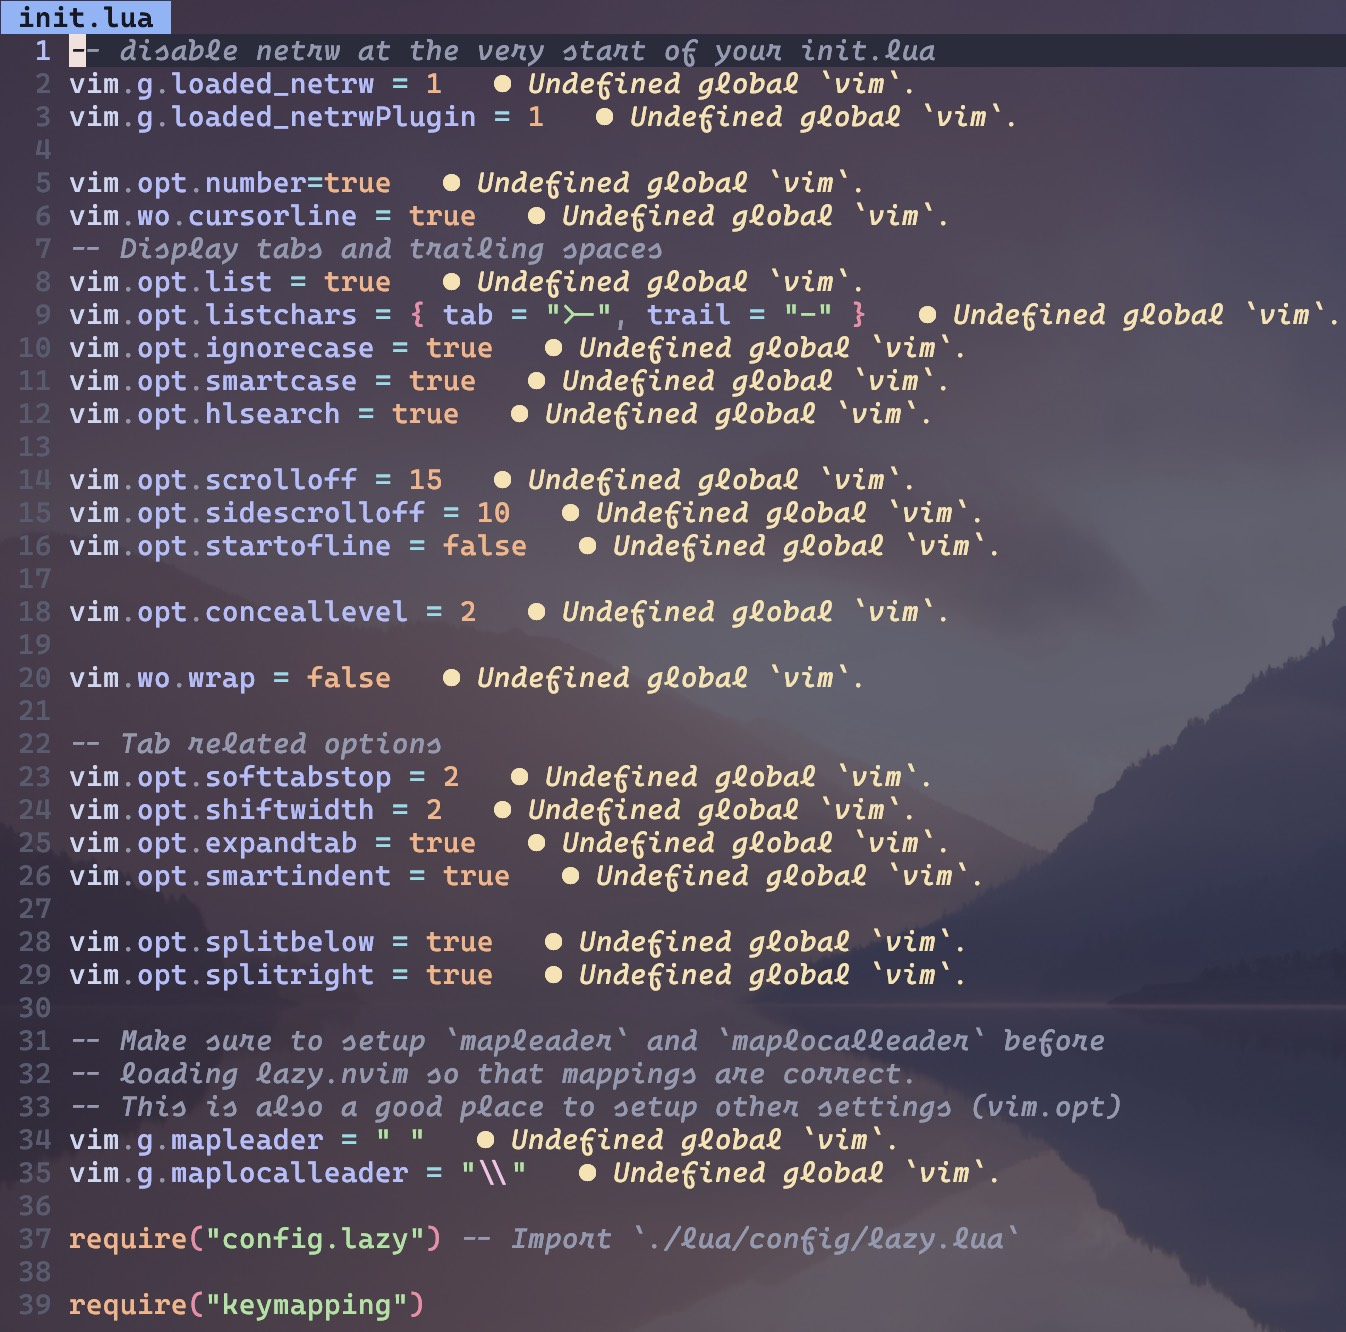
\includegraphics[width=0.6\linewidth]{./Figures/Lazydev_Before.jpg}
            \caption{安装之前}
          \end{figure}
        \end{column}

        \begin{column}{0.5\linewidth}
          \begin{figure}[H]
            \centering
            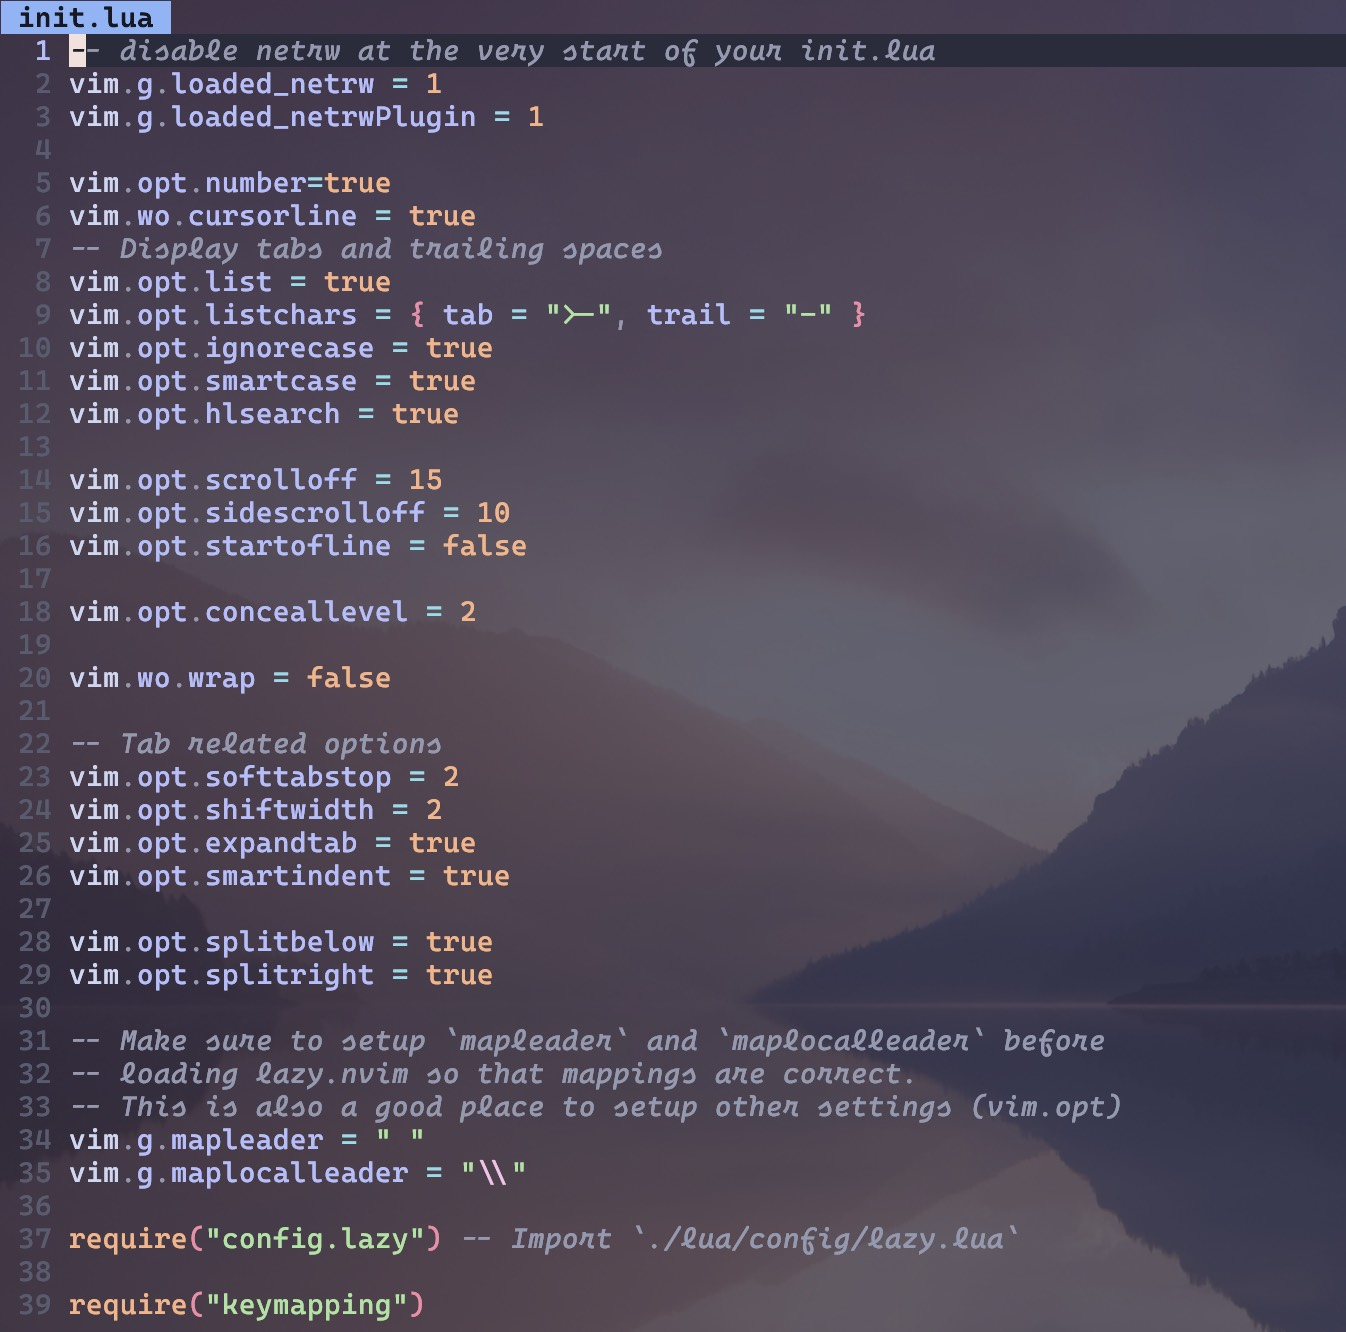
\includegraphics[width=0.6\linewidth]{./Figures/Lazydev_After.jpg}
            \caption{安装之后}
          \end{figure}
        \end{column}
      \end{columns}
    \end{frame}

  \subsection{which-key.nvim}
    \begin{frame}{which-key.nvim}
      显示快捷键

      \begin{figure}[H]
        \centering
        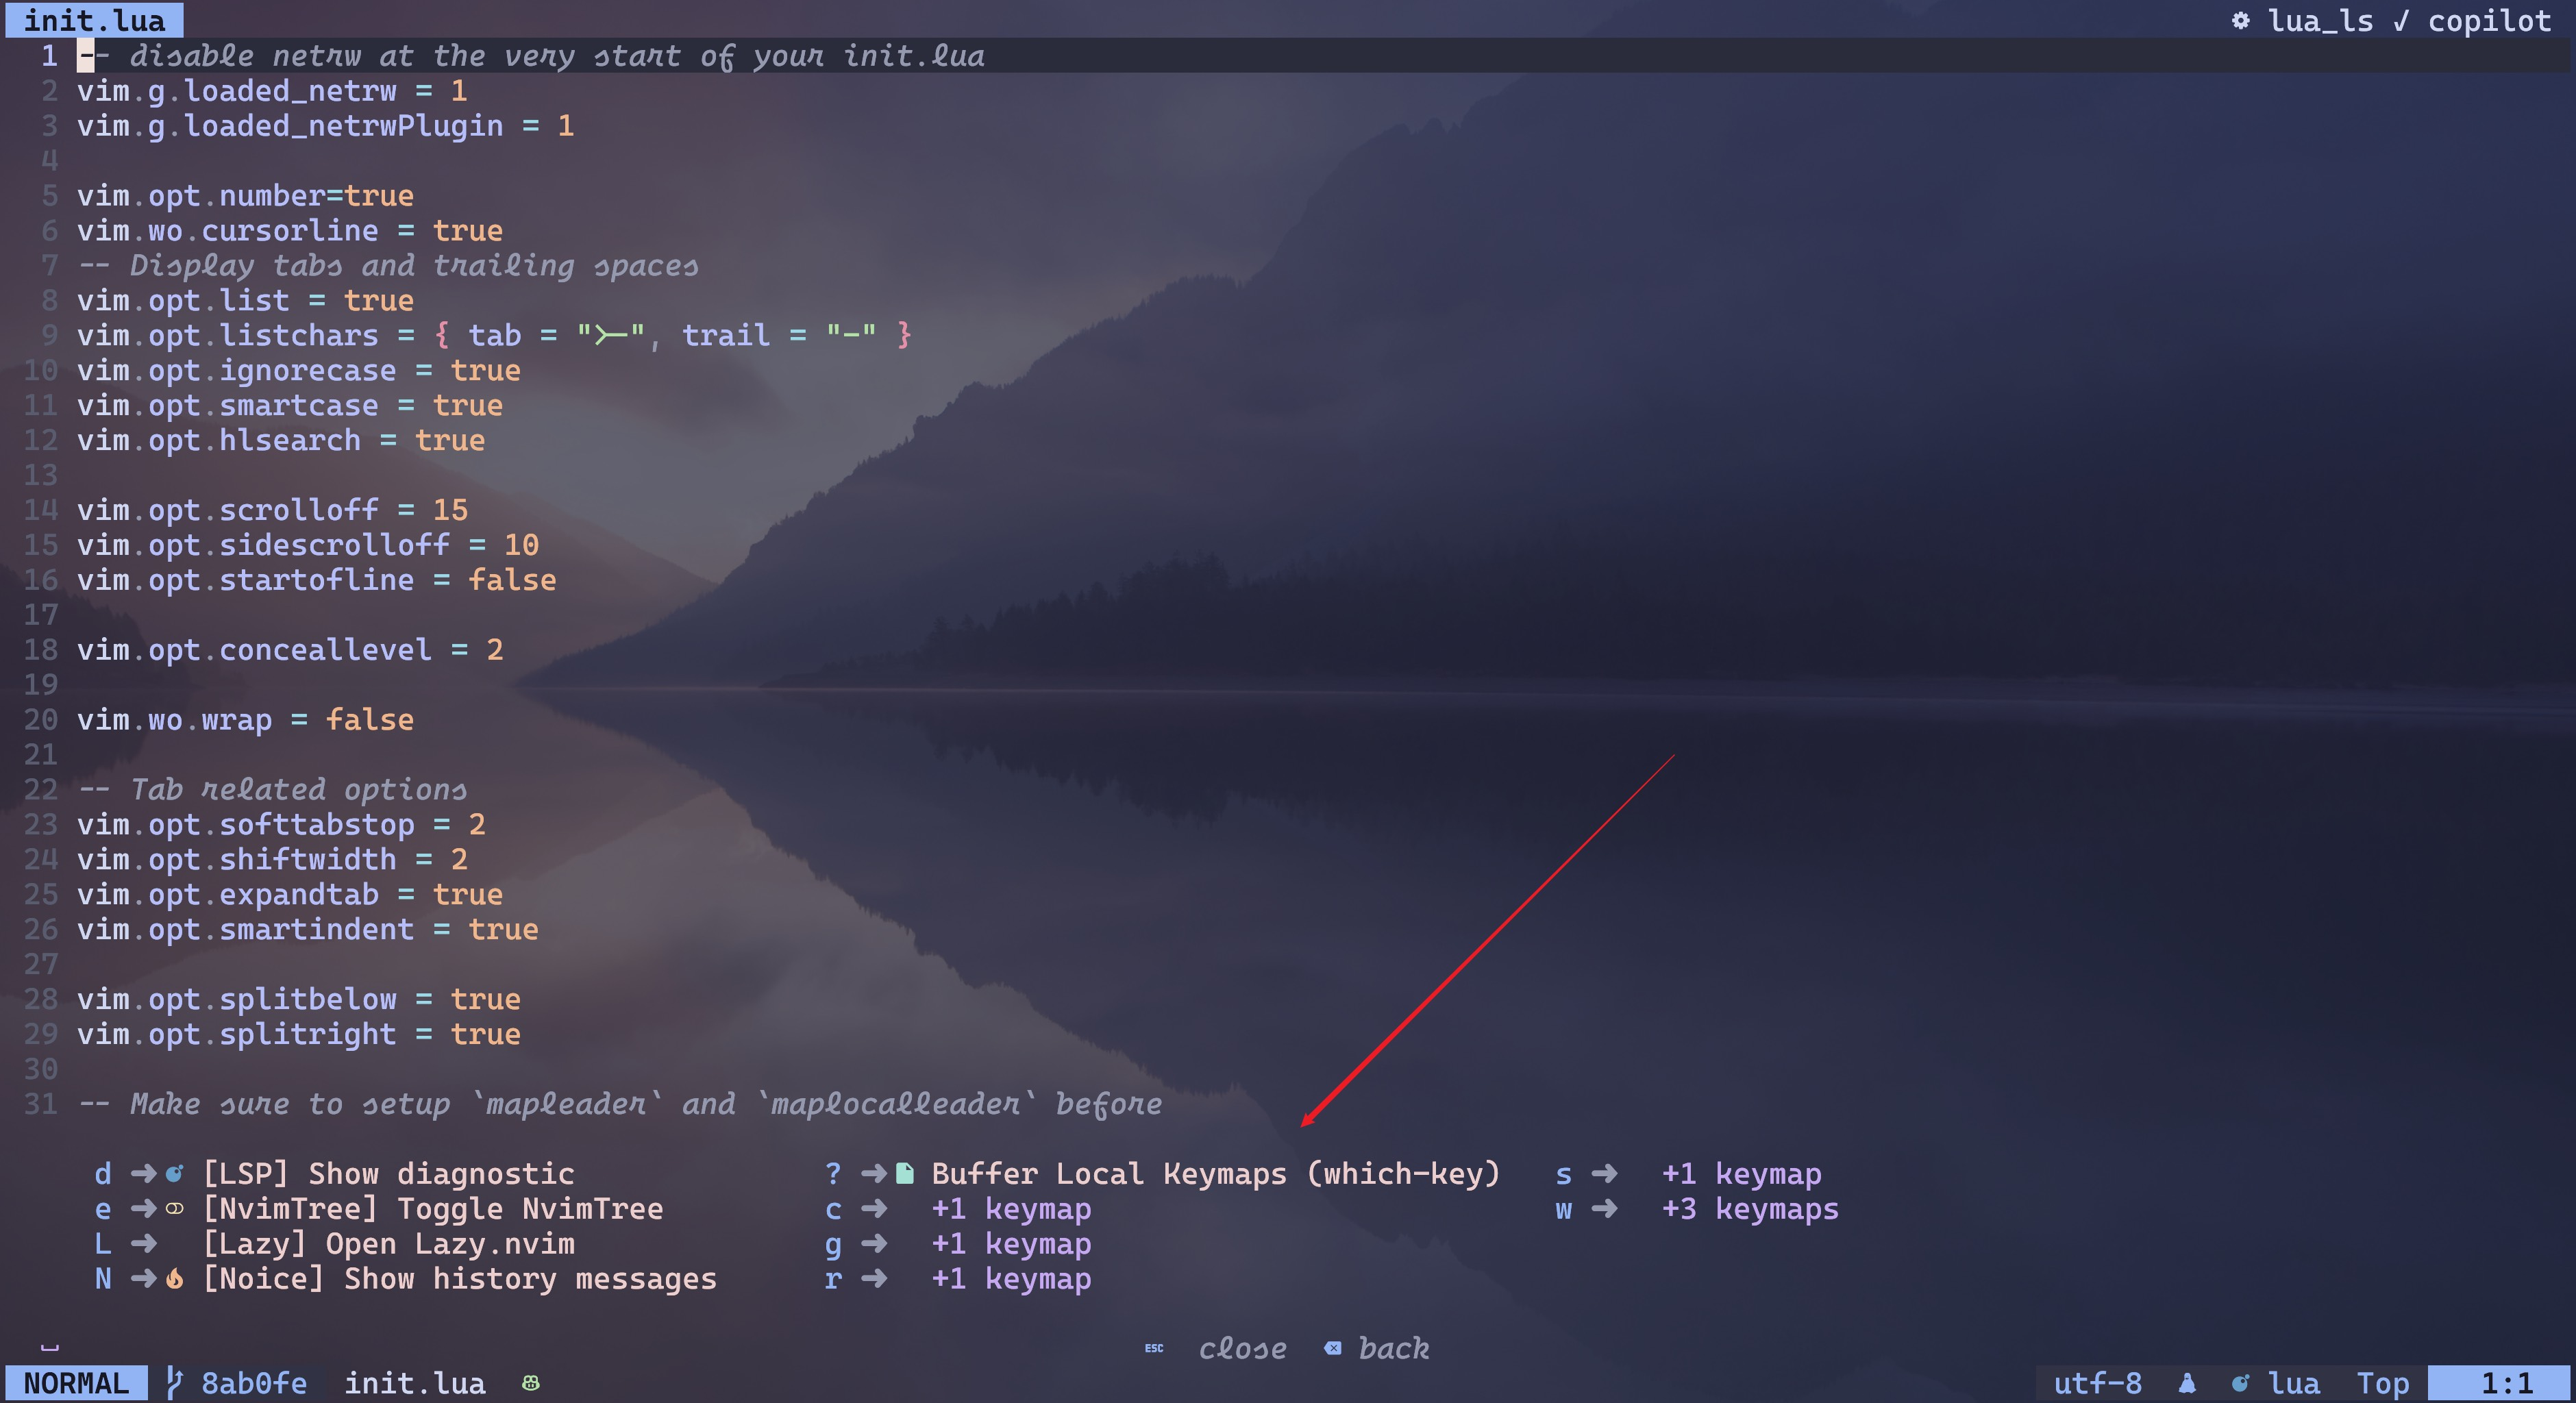
\includegraphics[width=0.7\linewidth]{./Figures/Which-key_After.jpg}
      \end{figure}

    \end{frame}

  \subsection{snacks.nvim}
    \begin{frame}{snacks.nvim}
      很多功能(在配置部分详细描述)

      \begin{figure}[H]
        \centering
        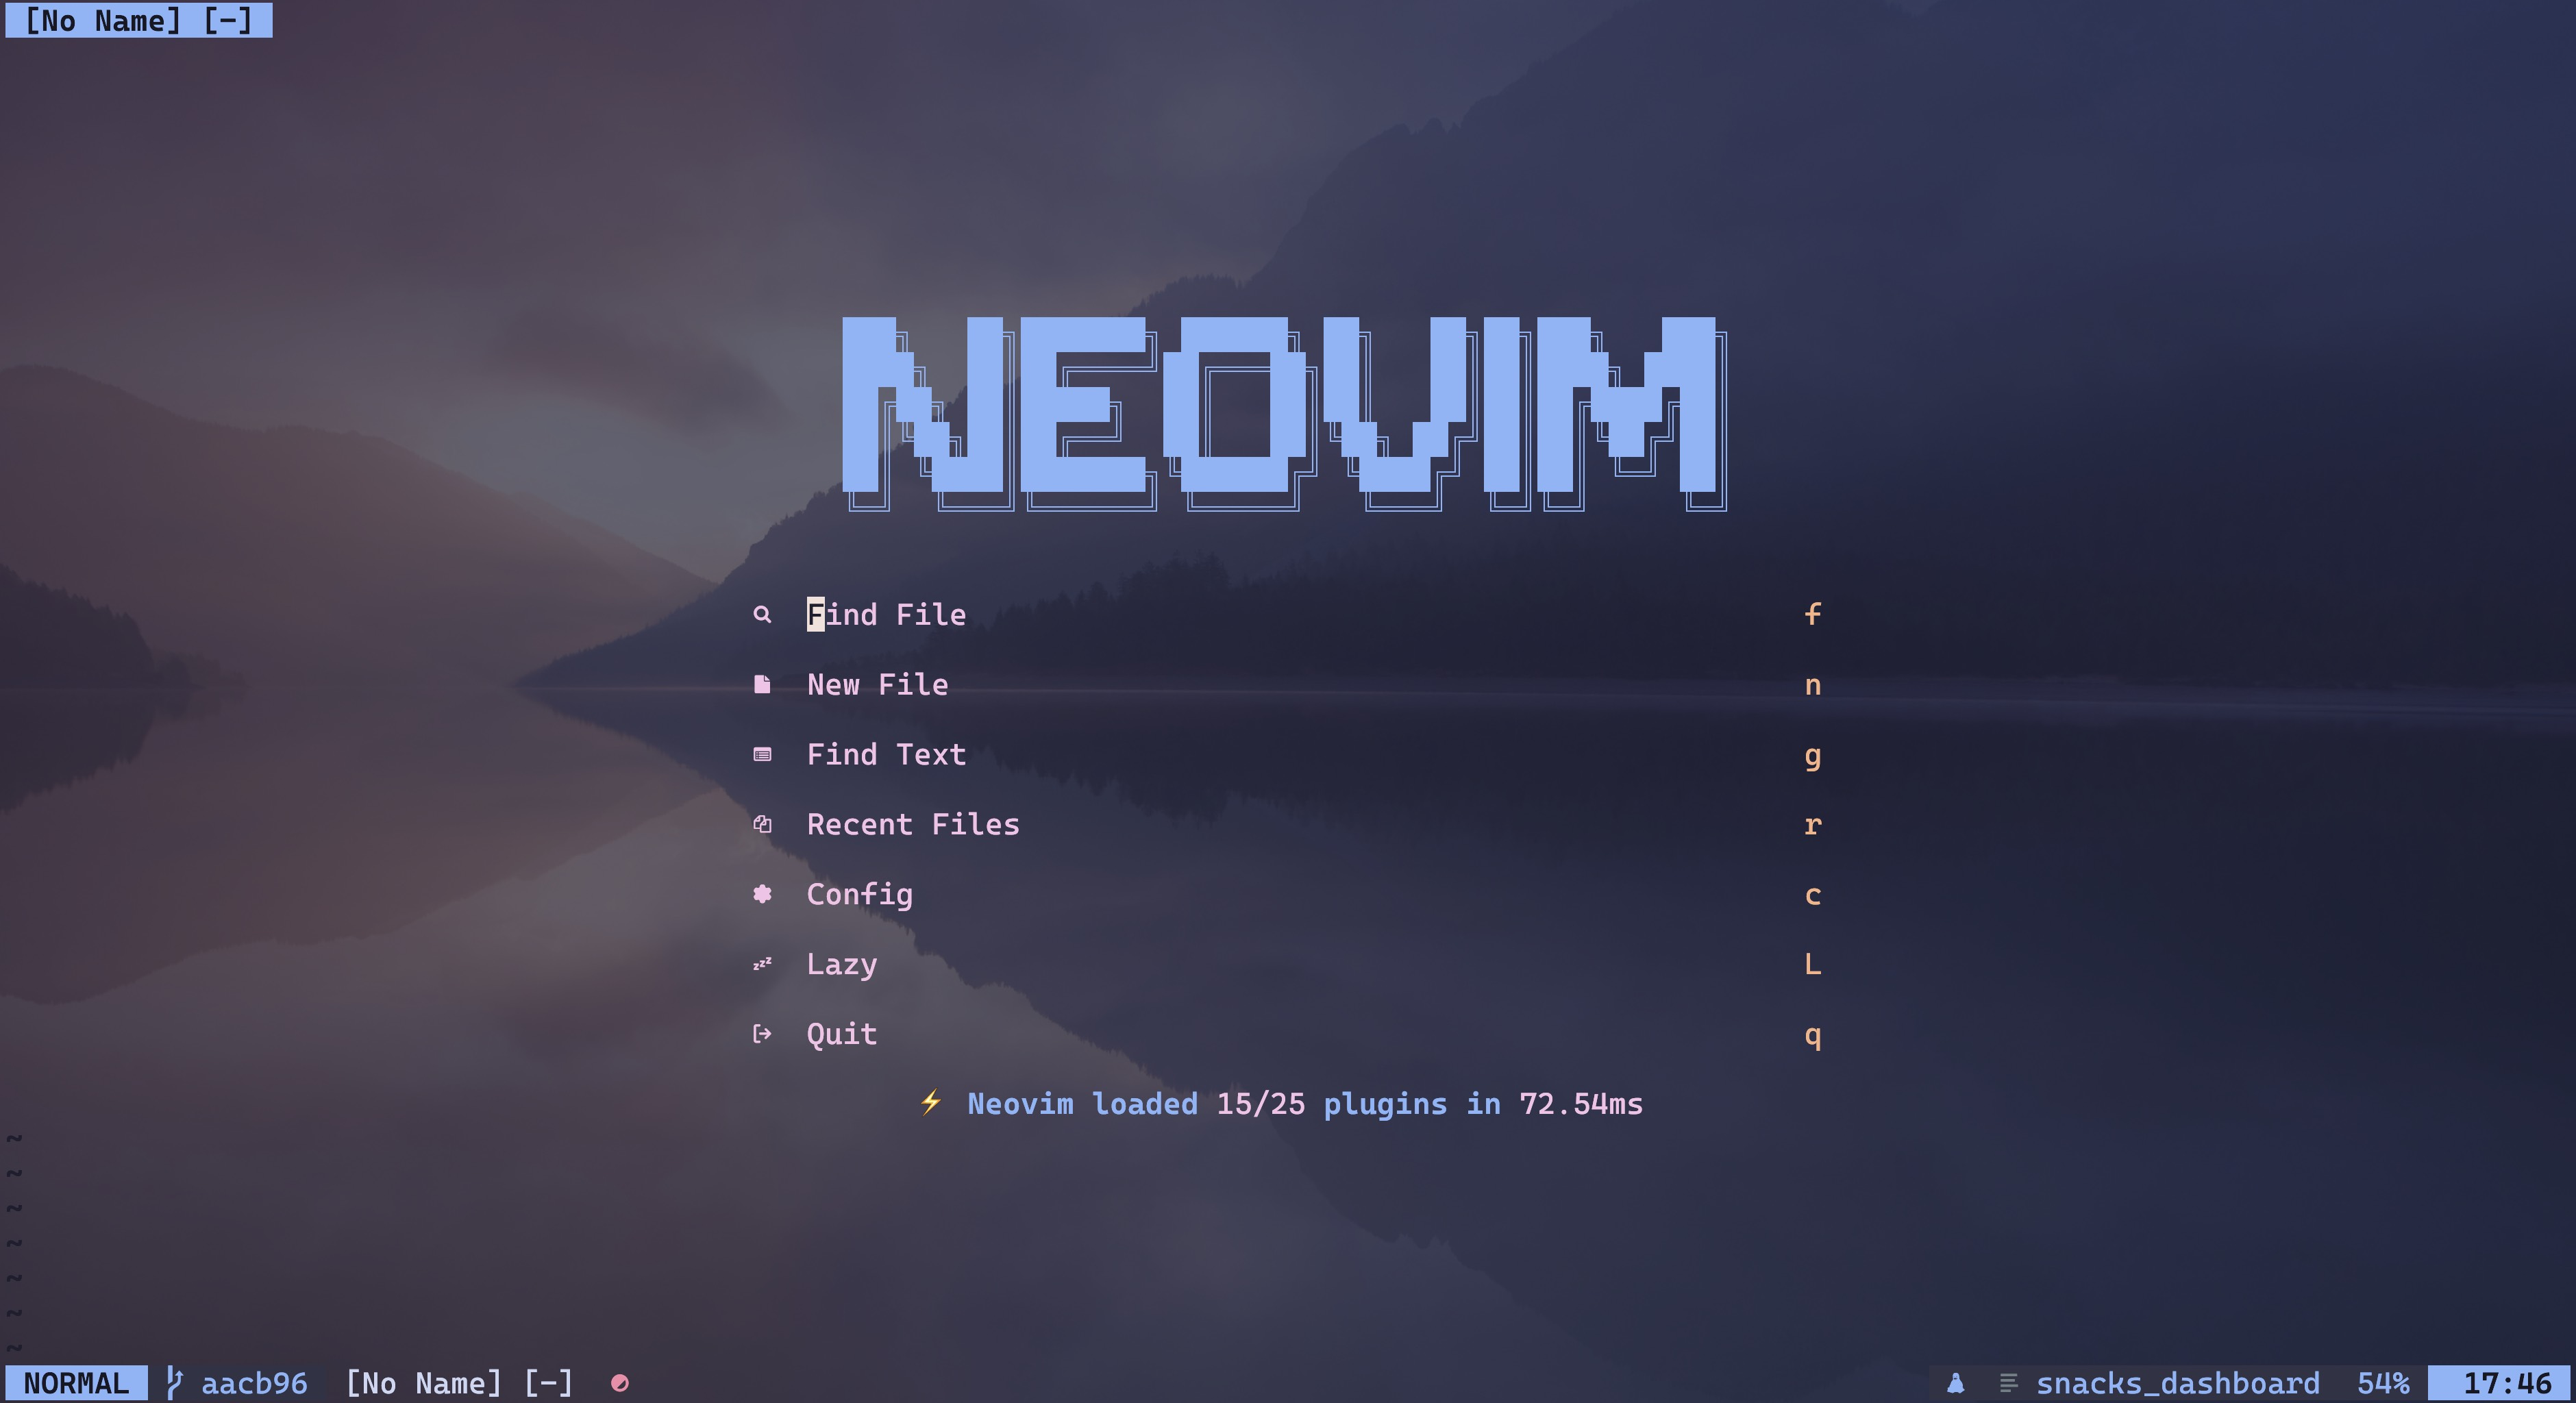
\includegraphics[width=0.7\linewidth]{./Figures/Snacks_After.jpg}
      \end{figure}

    \end{frame}

\section{插件配置}

  \begin{frame}{which-key.nvim}
    修改显示样式

    \begin{figure}[H]
      \centering
      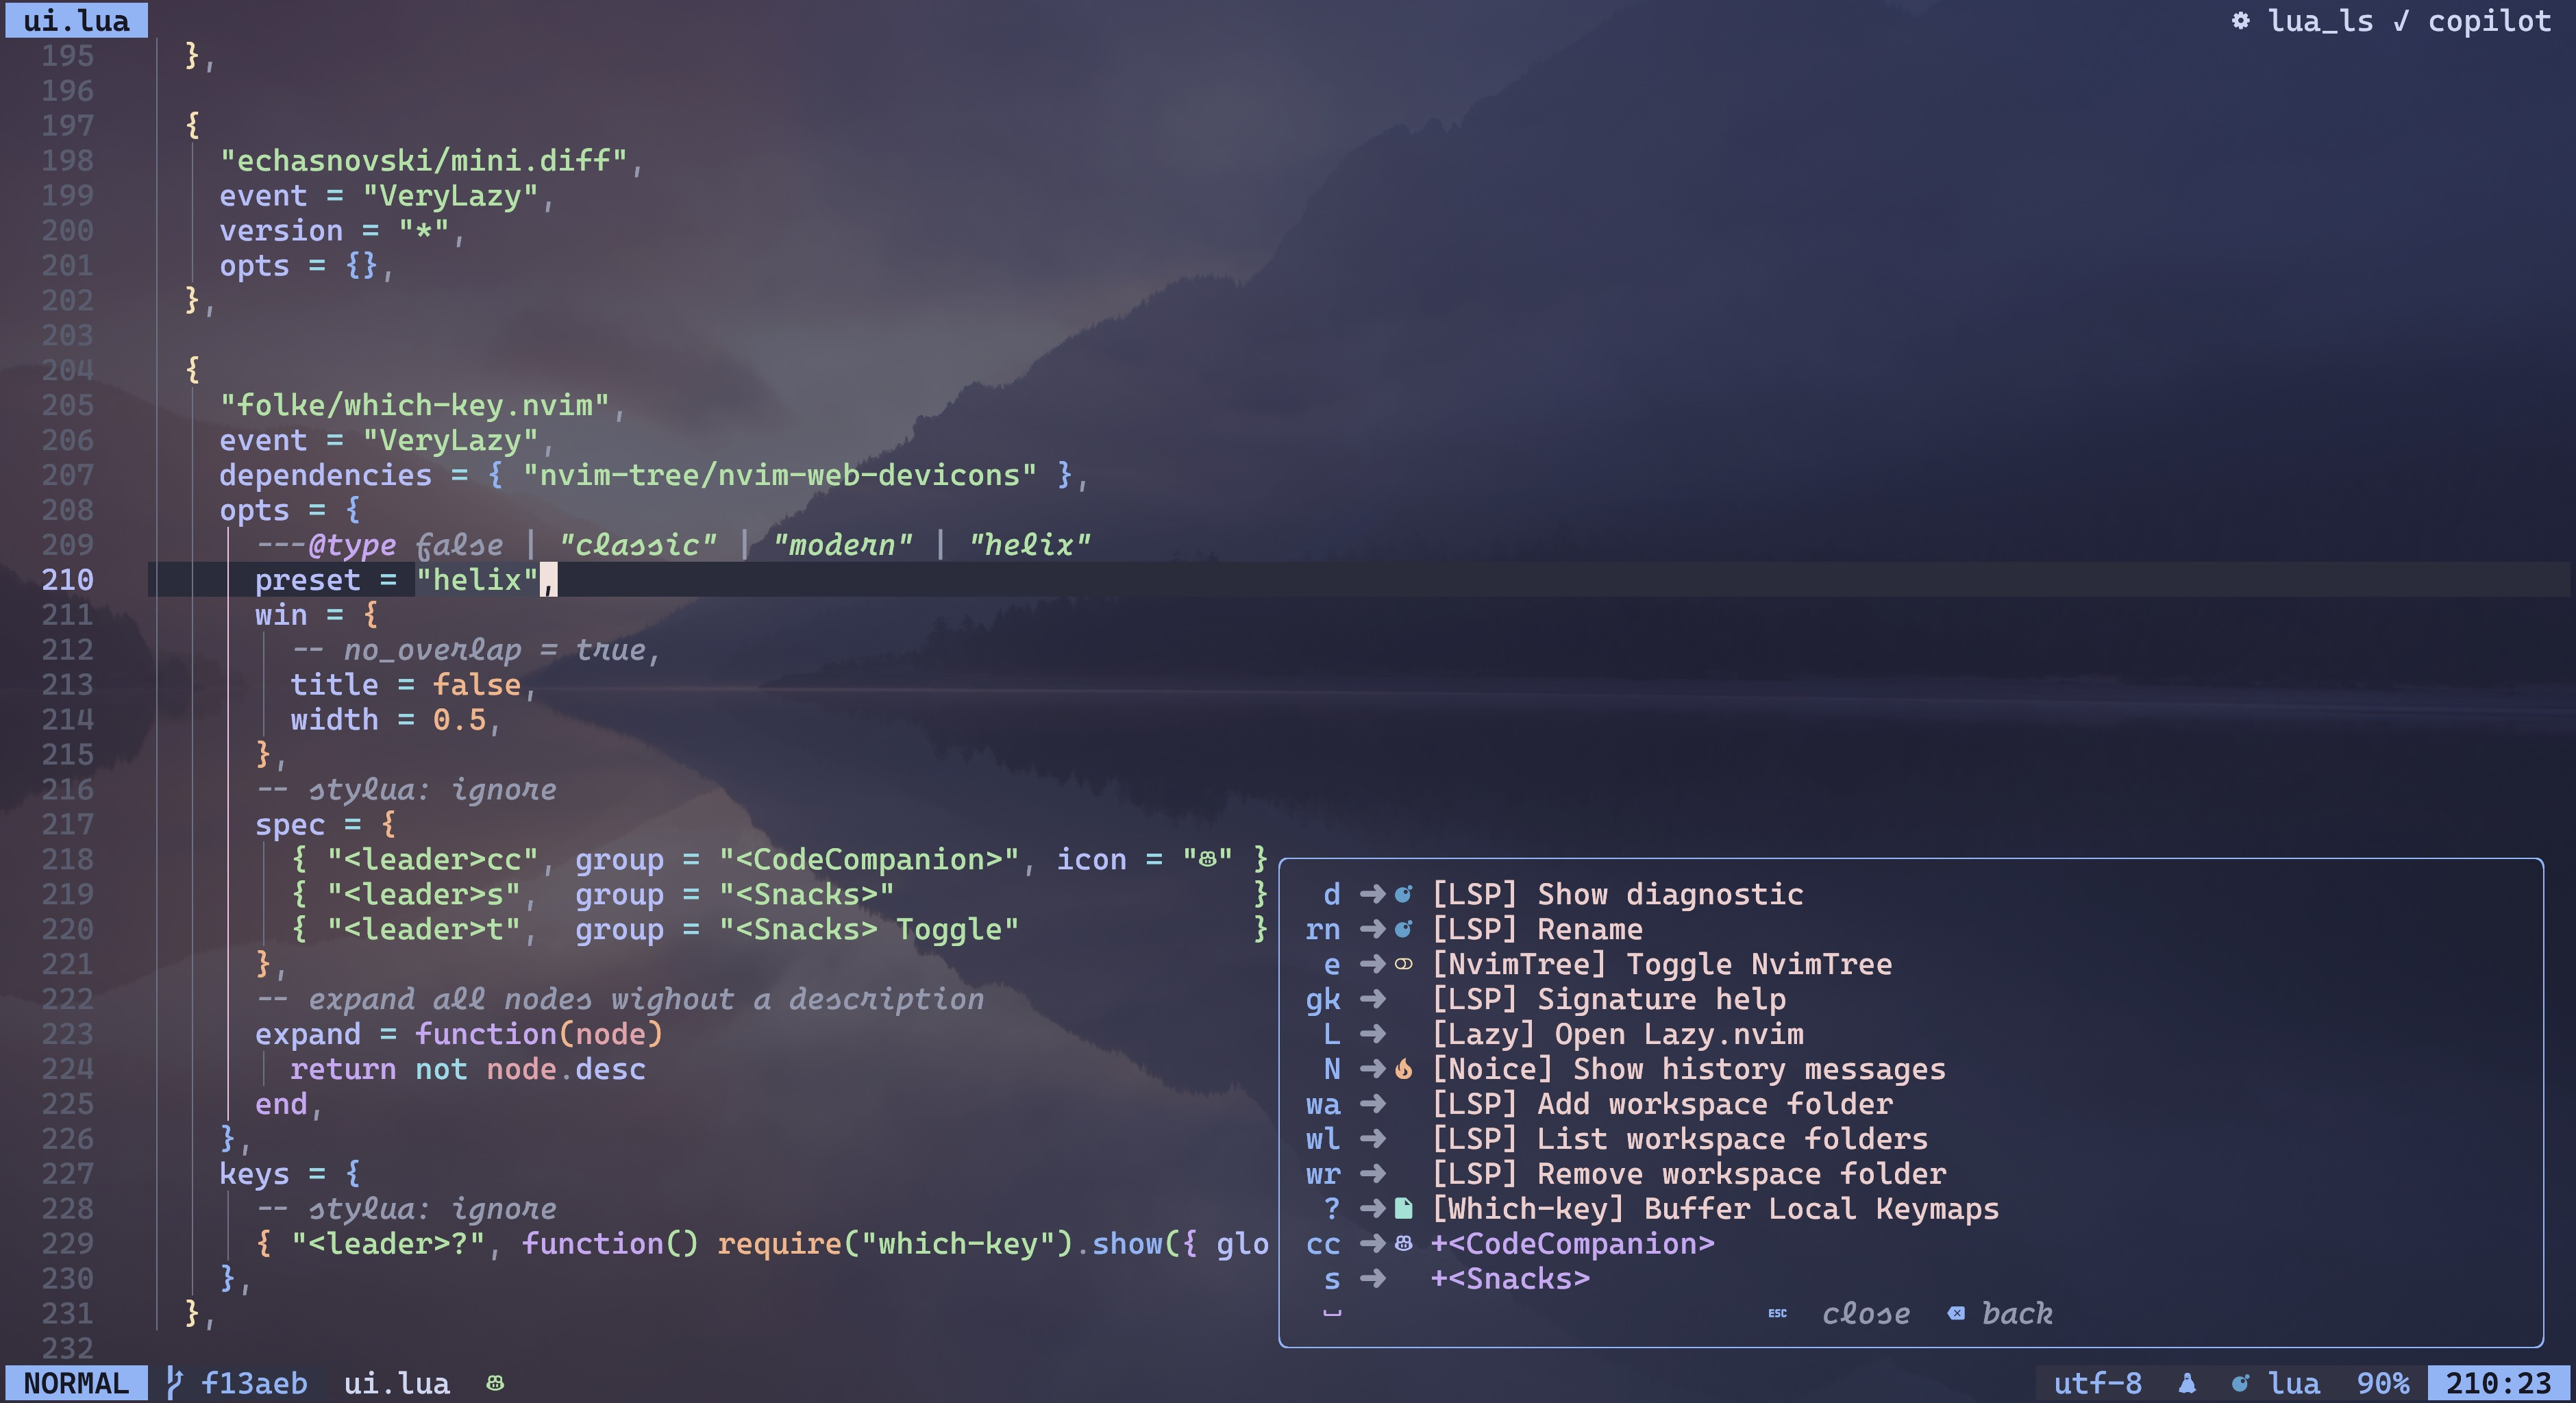
\includegraphics[width=0.7\linewidth]{./Figures/Which-key_Config.jpg}
    \end{figure}

  \end{frame}

  \begin{frame}{snacks.nvim}
    \begin{itemize}
      \item 添加功能切换快捷键,并且默认禁用动画
        \begin{figure}[H]
          \centering
          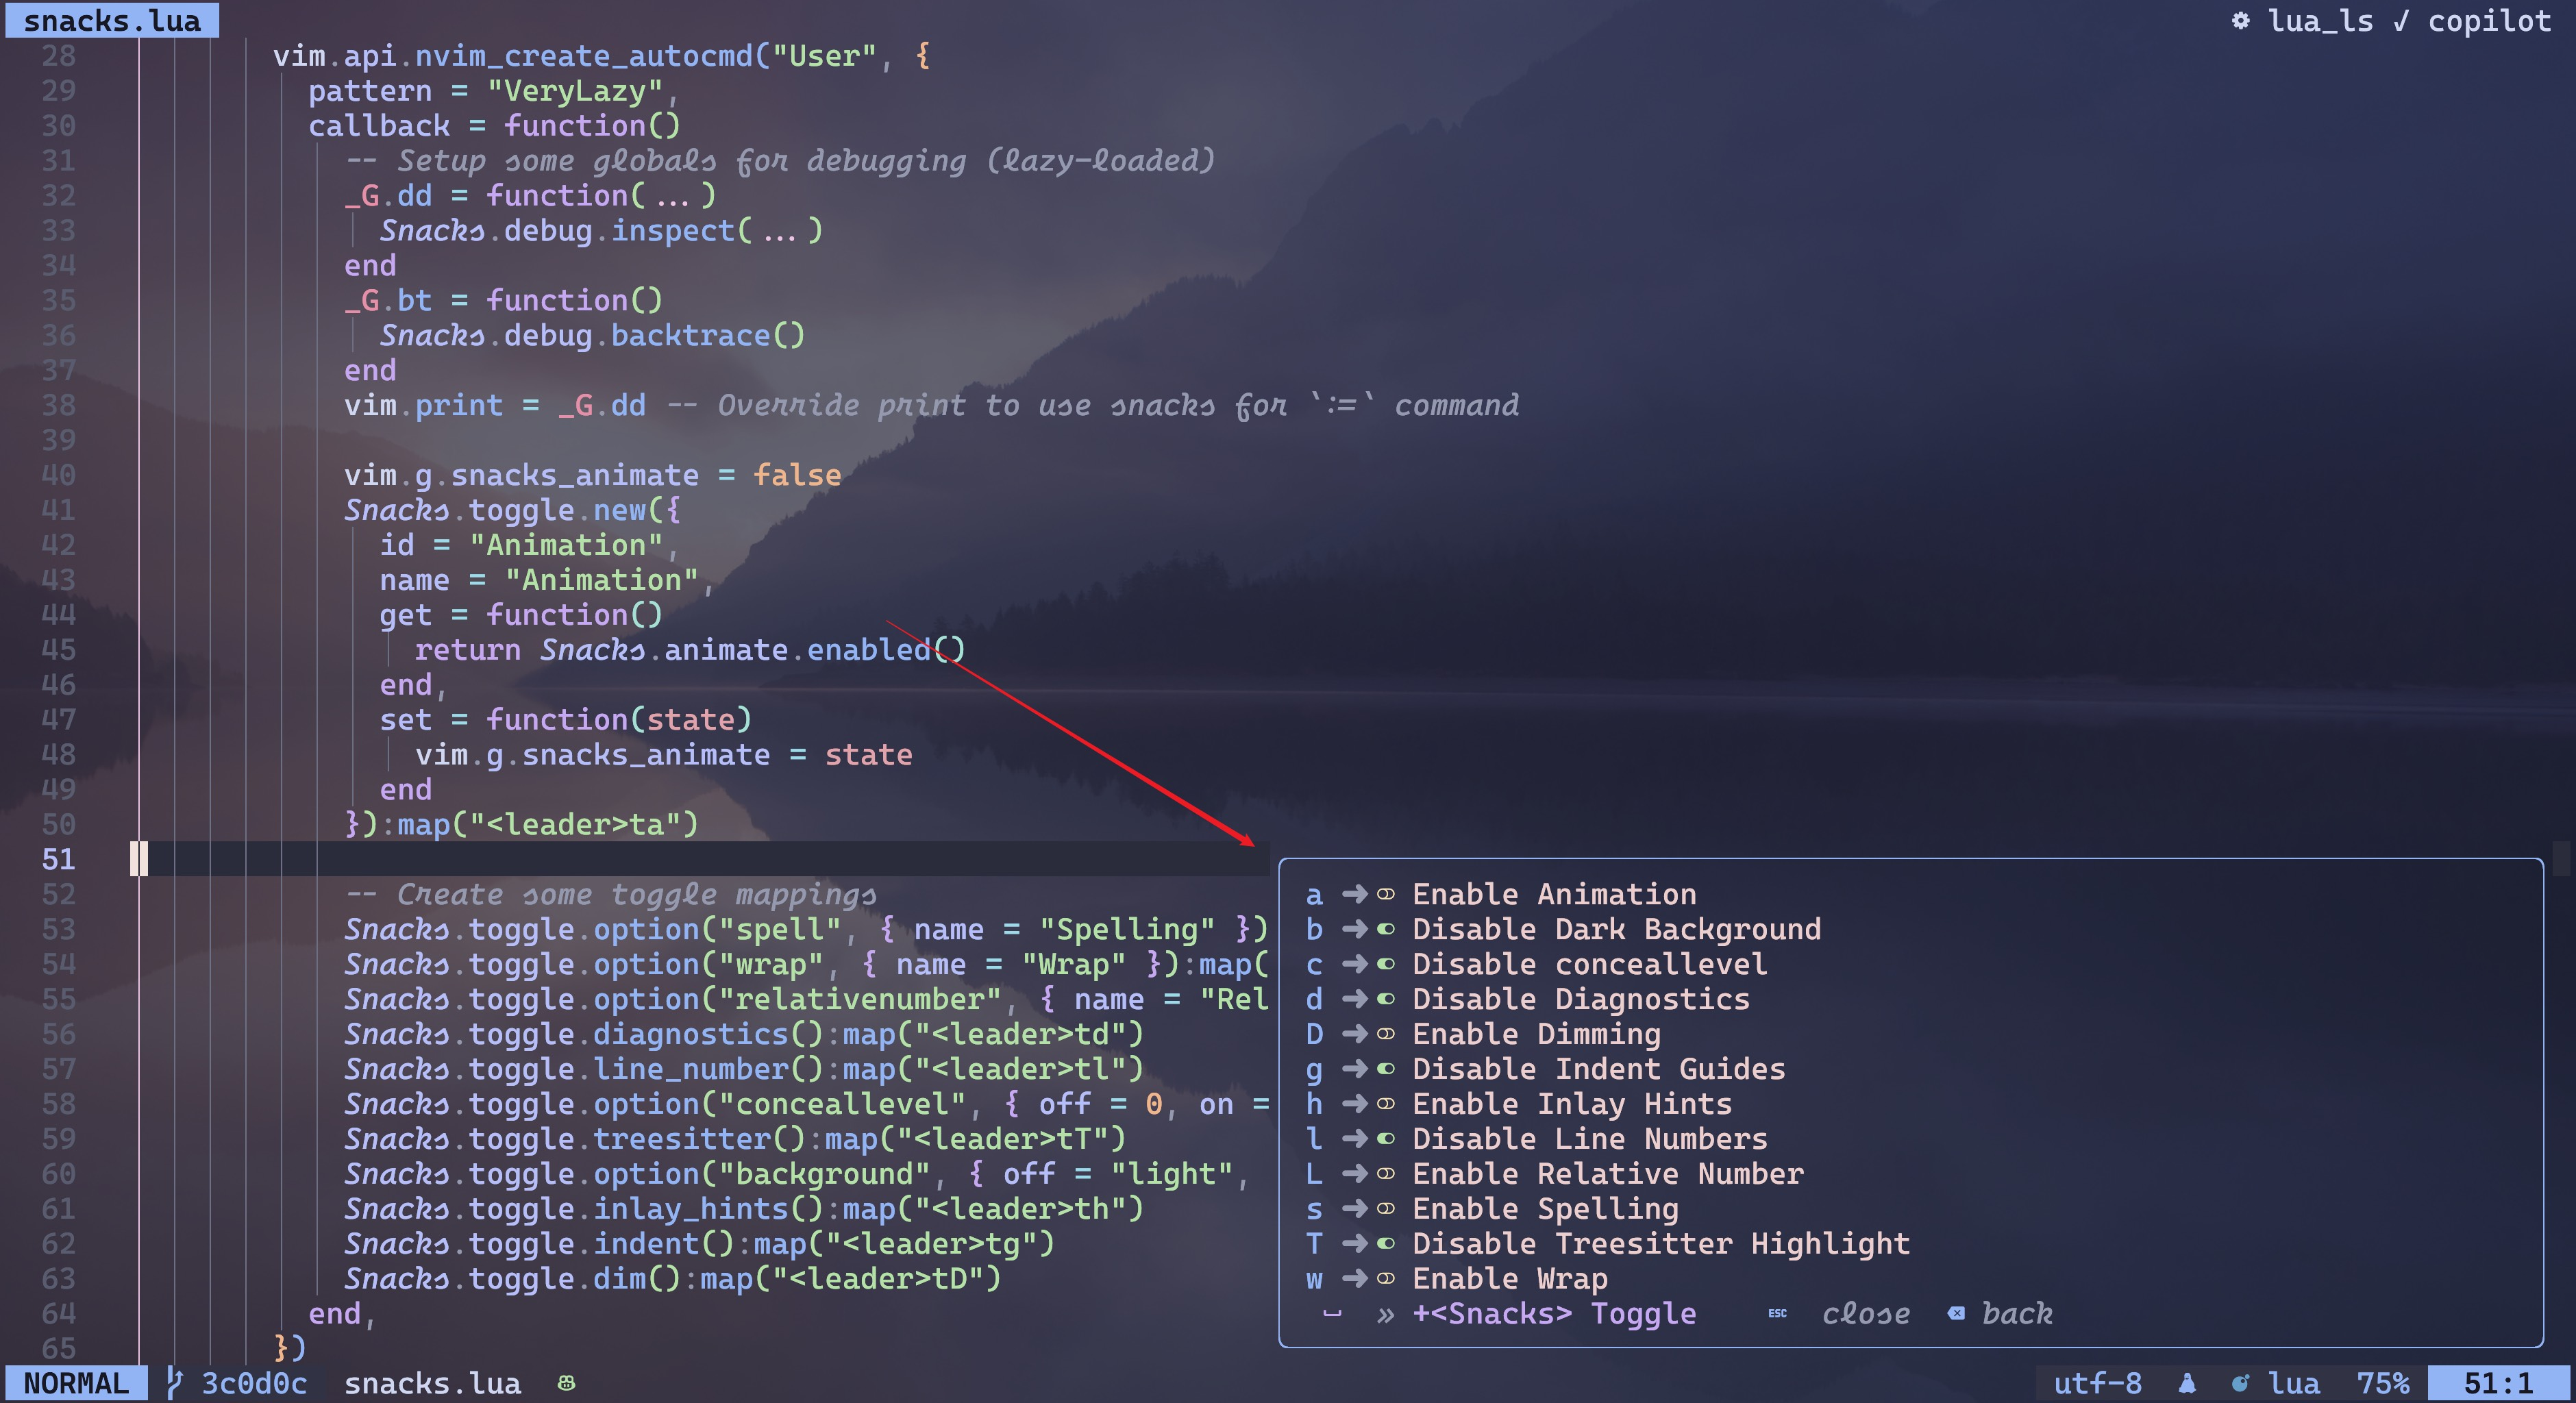
\includegraphics[width=0.7\linewidth]{./Figures/Snacks_Config_1_Toggle.jpg}
        \end{figure}
    \end{itemize}
  \end{frame}

  \begin{frame}{snacks.nvim}
    \begin{itemize}
      \item 暗淡不活跃代码 % ChkTeX 19
        \begin{figure}[H]
          \centering
          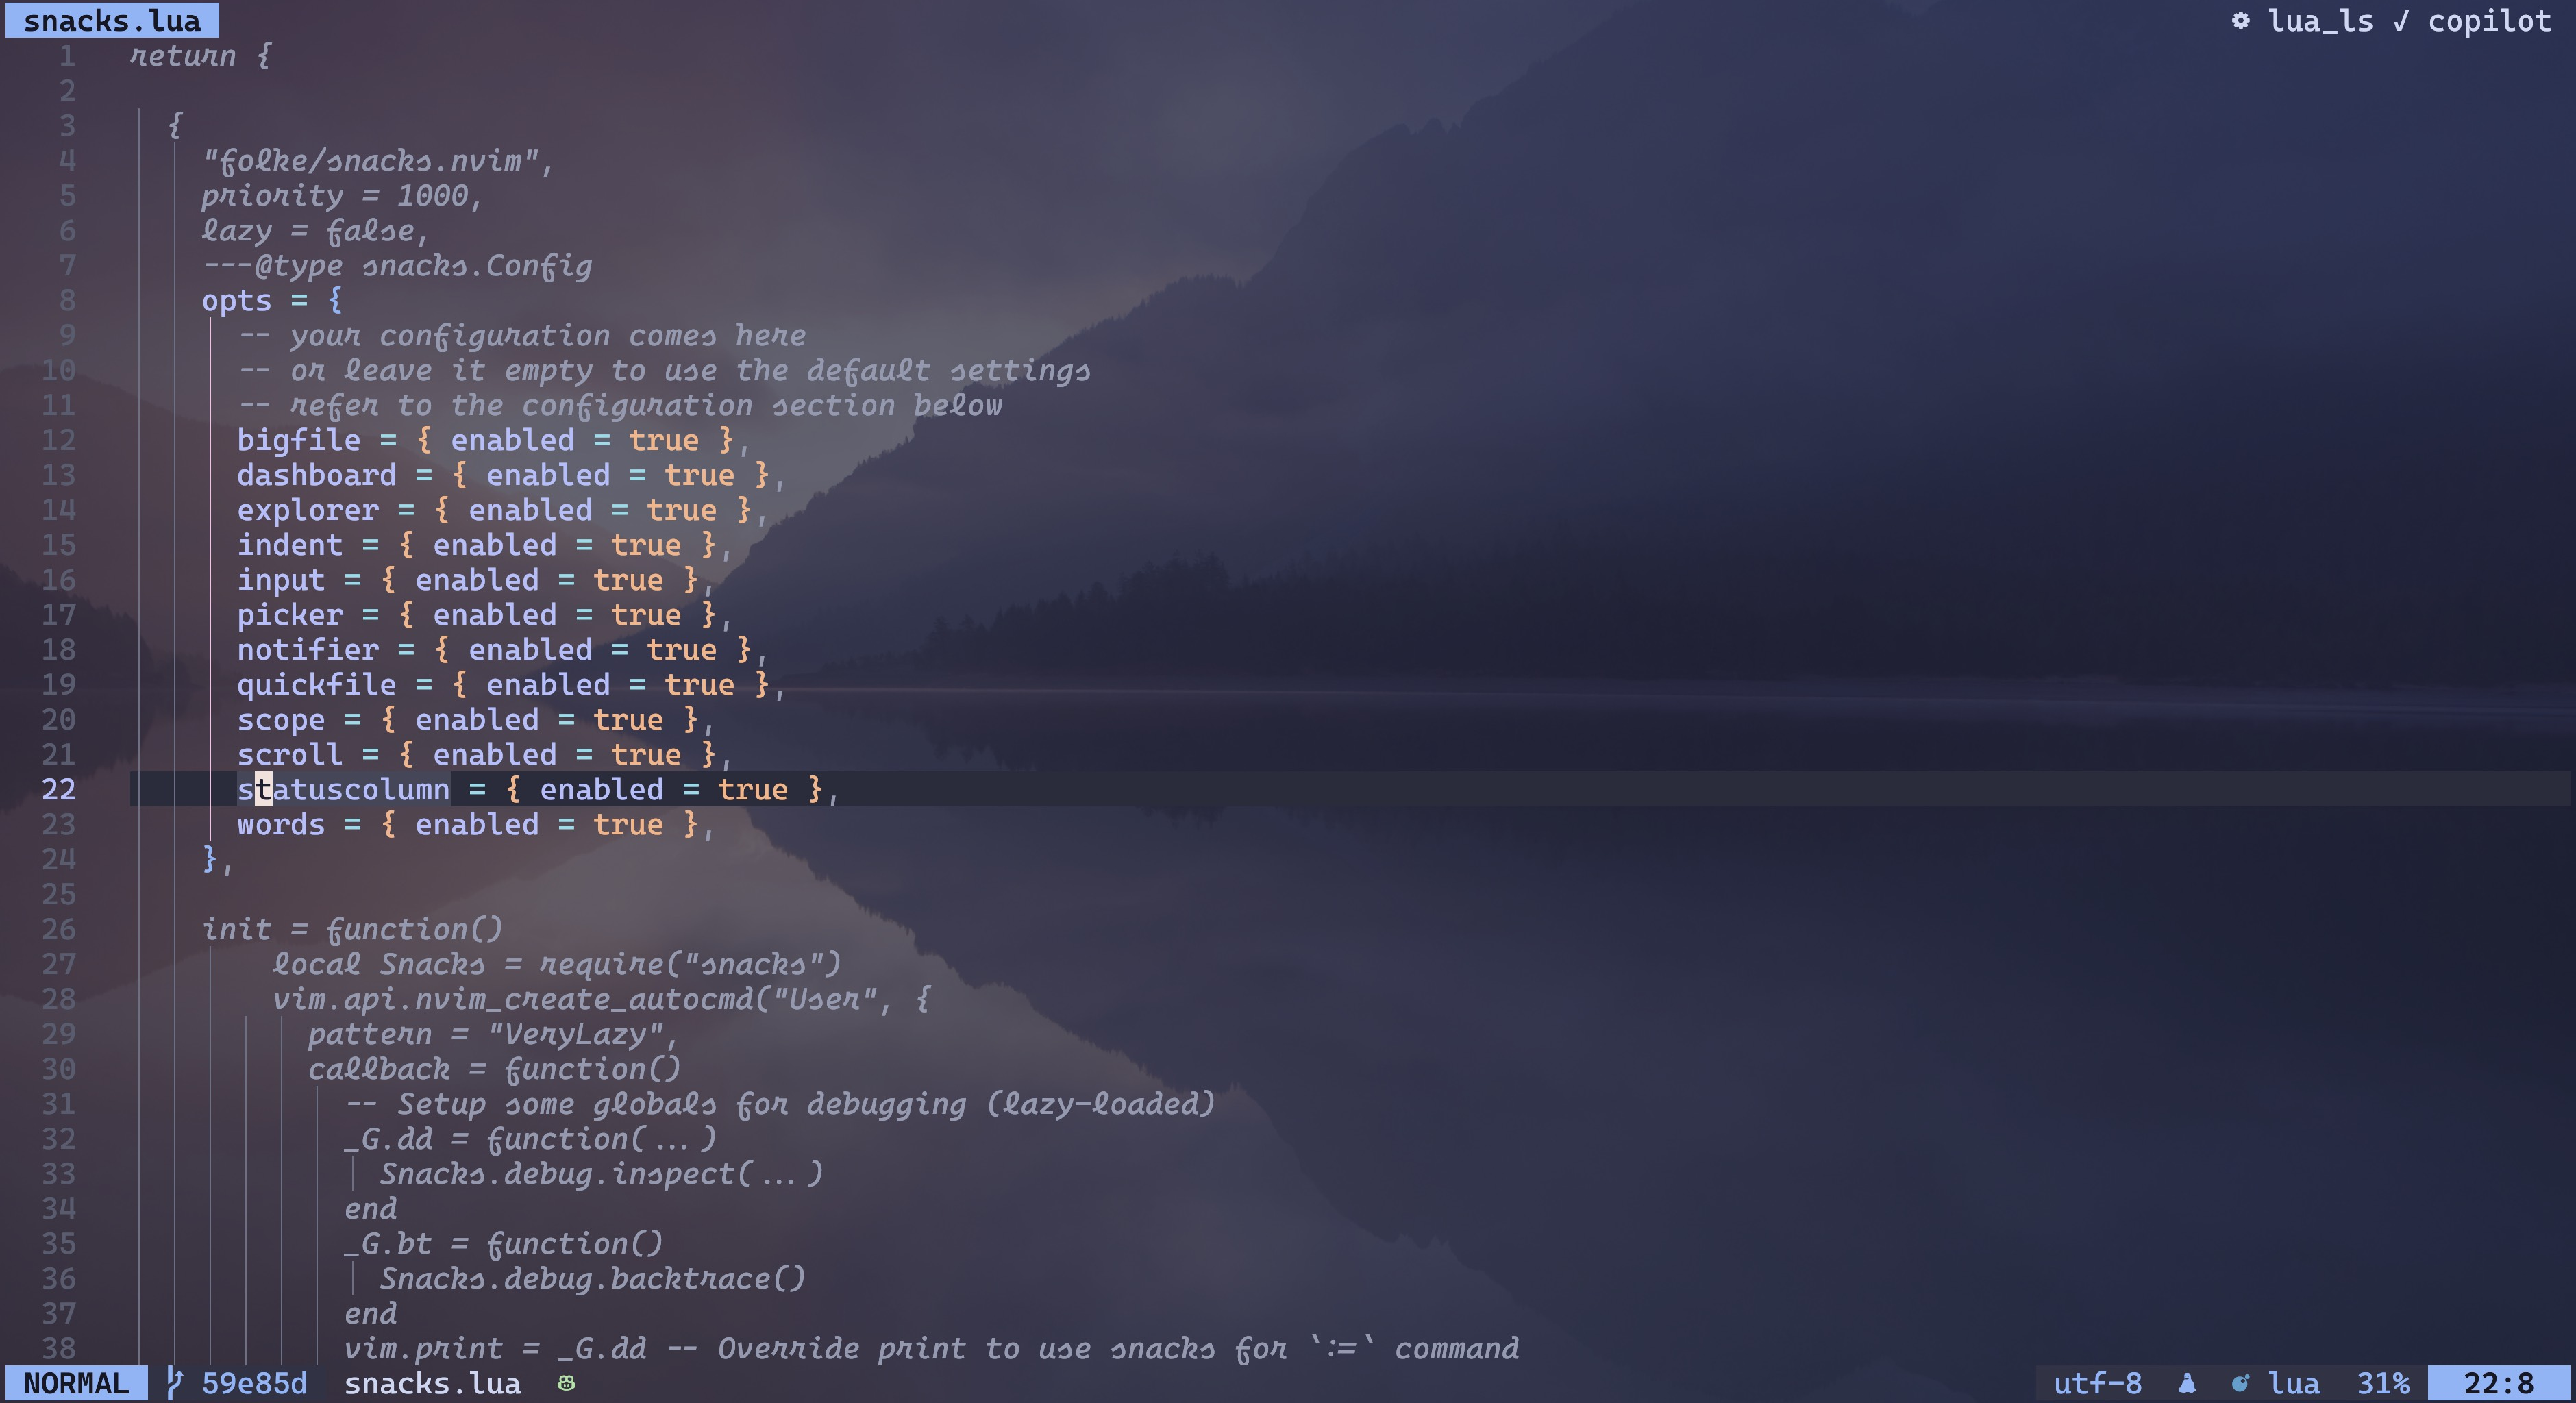
\includegraphics[width=0.7\linewidth]{./Figures/Snacks_Config_2_Dim.jpg}
        \end{figure}
    \end{itemize}
  \end{frame}

  \begin{frame}{snacks.nvim}
    \begin{itemize}
      \item 关闭文件的快捷键
      \item 关闭文件管理器的功能(我们用nvim-tree.lua)
      \item 添加Git相关的快捷键(git blame和git browse)
    \end{itemize}
  \end{frame}

  \begin{frame}{snacks.nvim}
    \begin{itemize}
      \item 显示图片
        \begin{itemize}
          \item 前置条件
            \begin{itemize}
              \item 支持\link{Kitty Graphics Protocol}{https://sw.kovidgoyal.net/kitty/graphics-protocol/}的终端(如kitty, ghostty, wezterm等)
              \item imagemagick:图片转换
              \item tectonic:LaTeX公式渲染
            \end{itemize}
          \item 使用 \lstinline[style=nvim]{:checkhealth snacks} 确认条件是否满足
        \end{itemize}
        \begin{figure}[H]
          \centering
          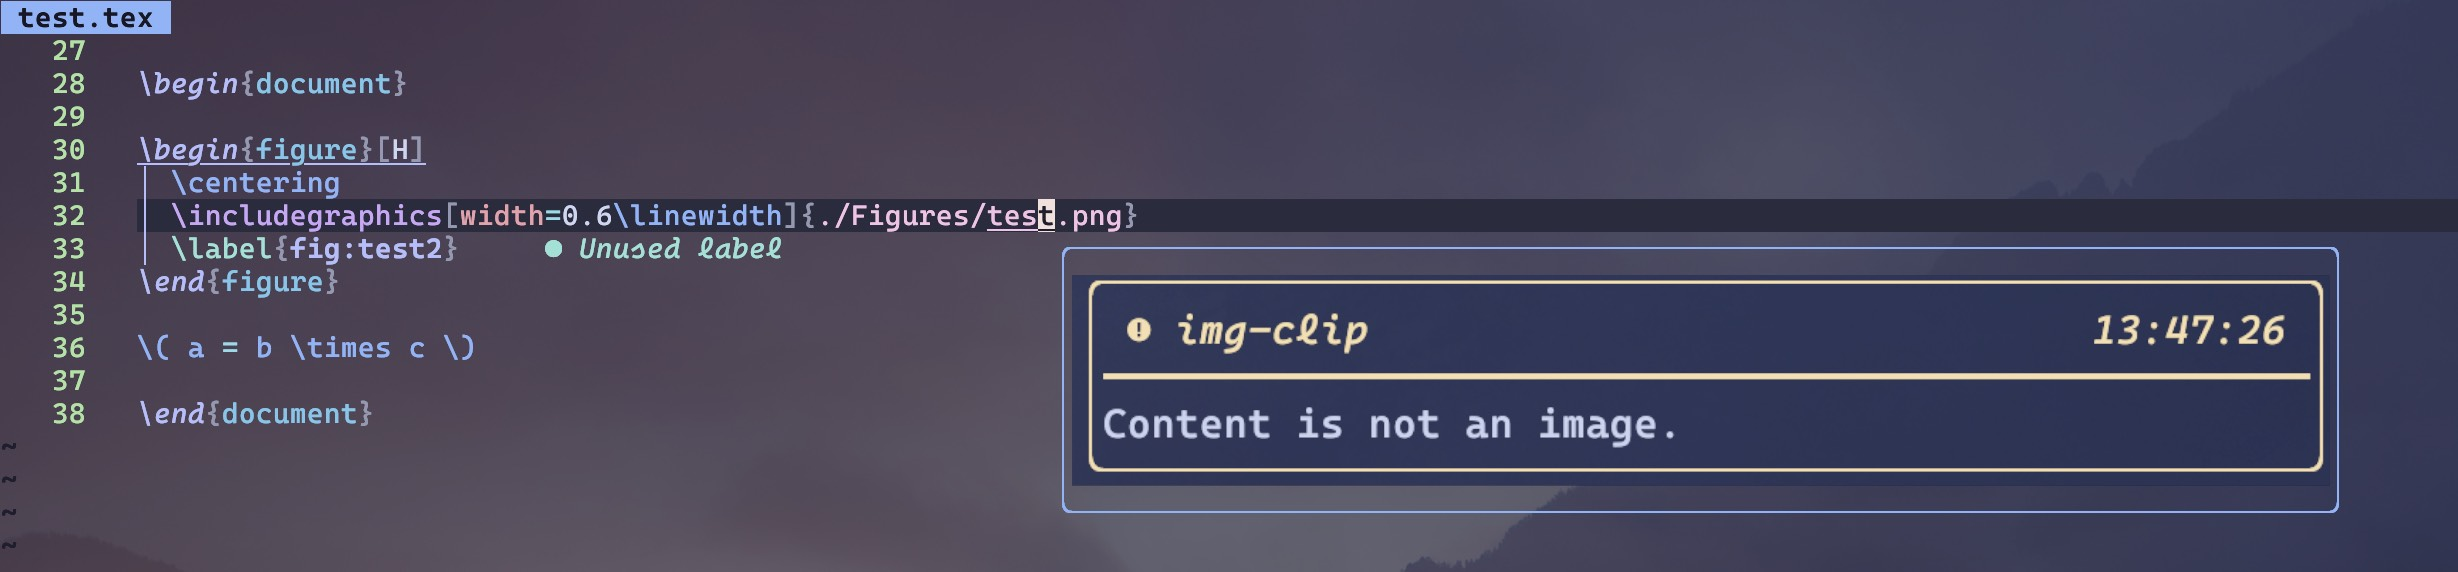
\includegraphics[width=0.9\linewidth]{./Figures/Snacks_Config_3_Image.jpg}
        \end{figure}
    \end{itemize}
  \end{frame}

  \begin{frame}{snacks.nvim}
    \begin{itemize}
      \item 显示代码缩进
        \begin{figure}[H]
          \centering
          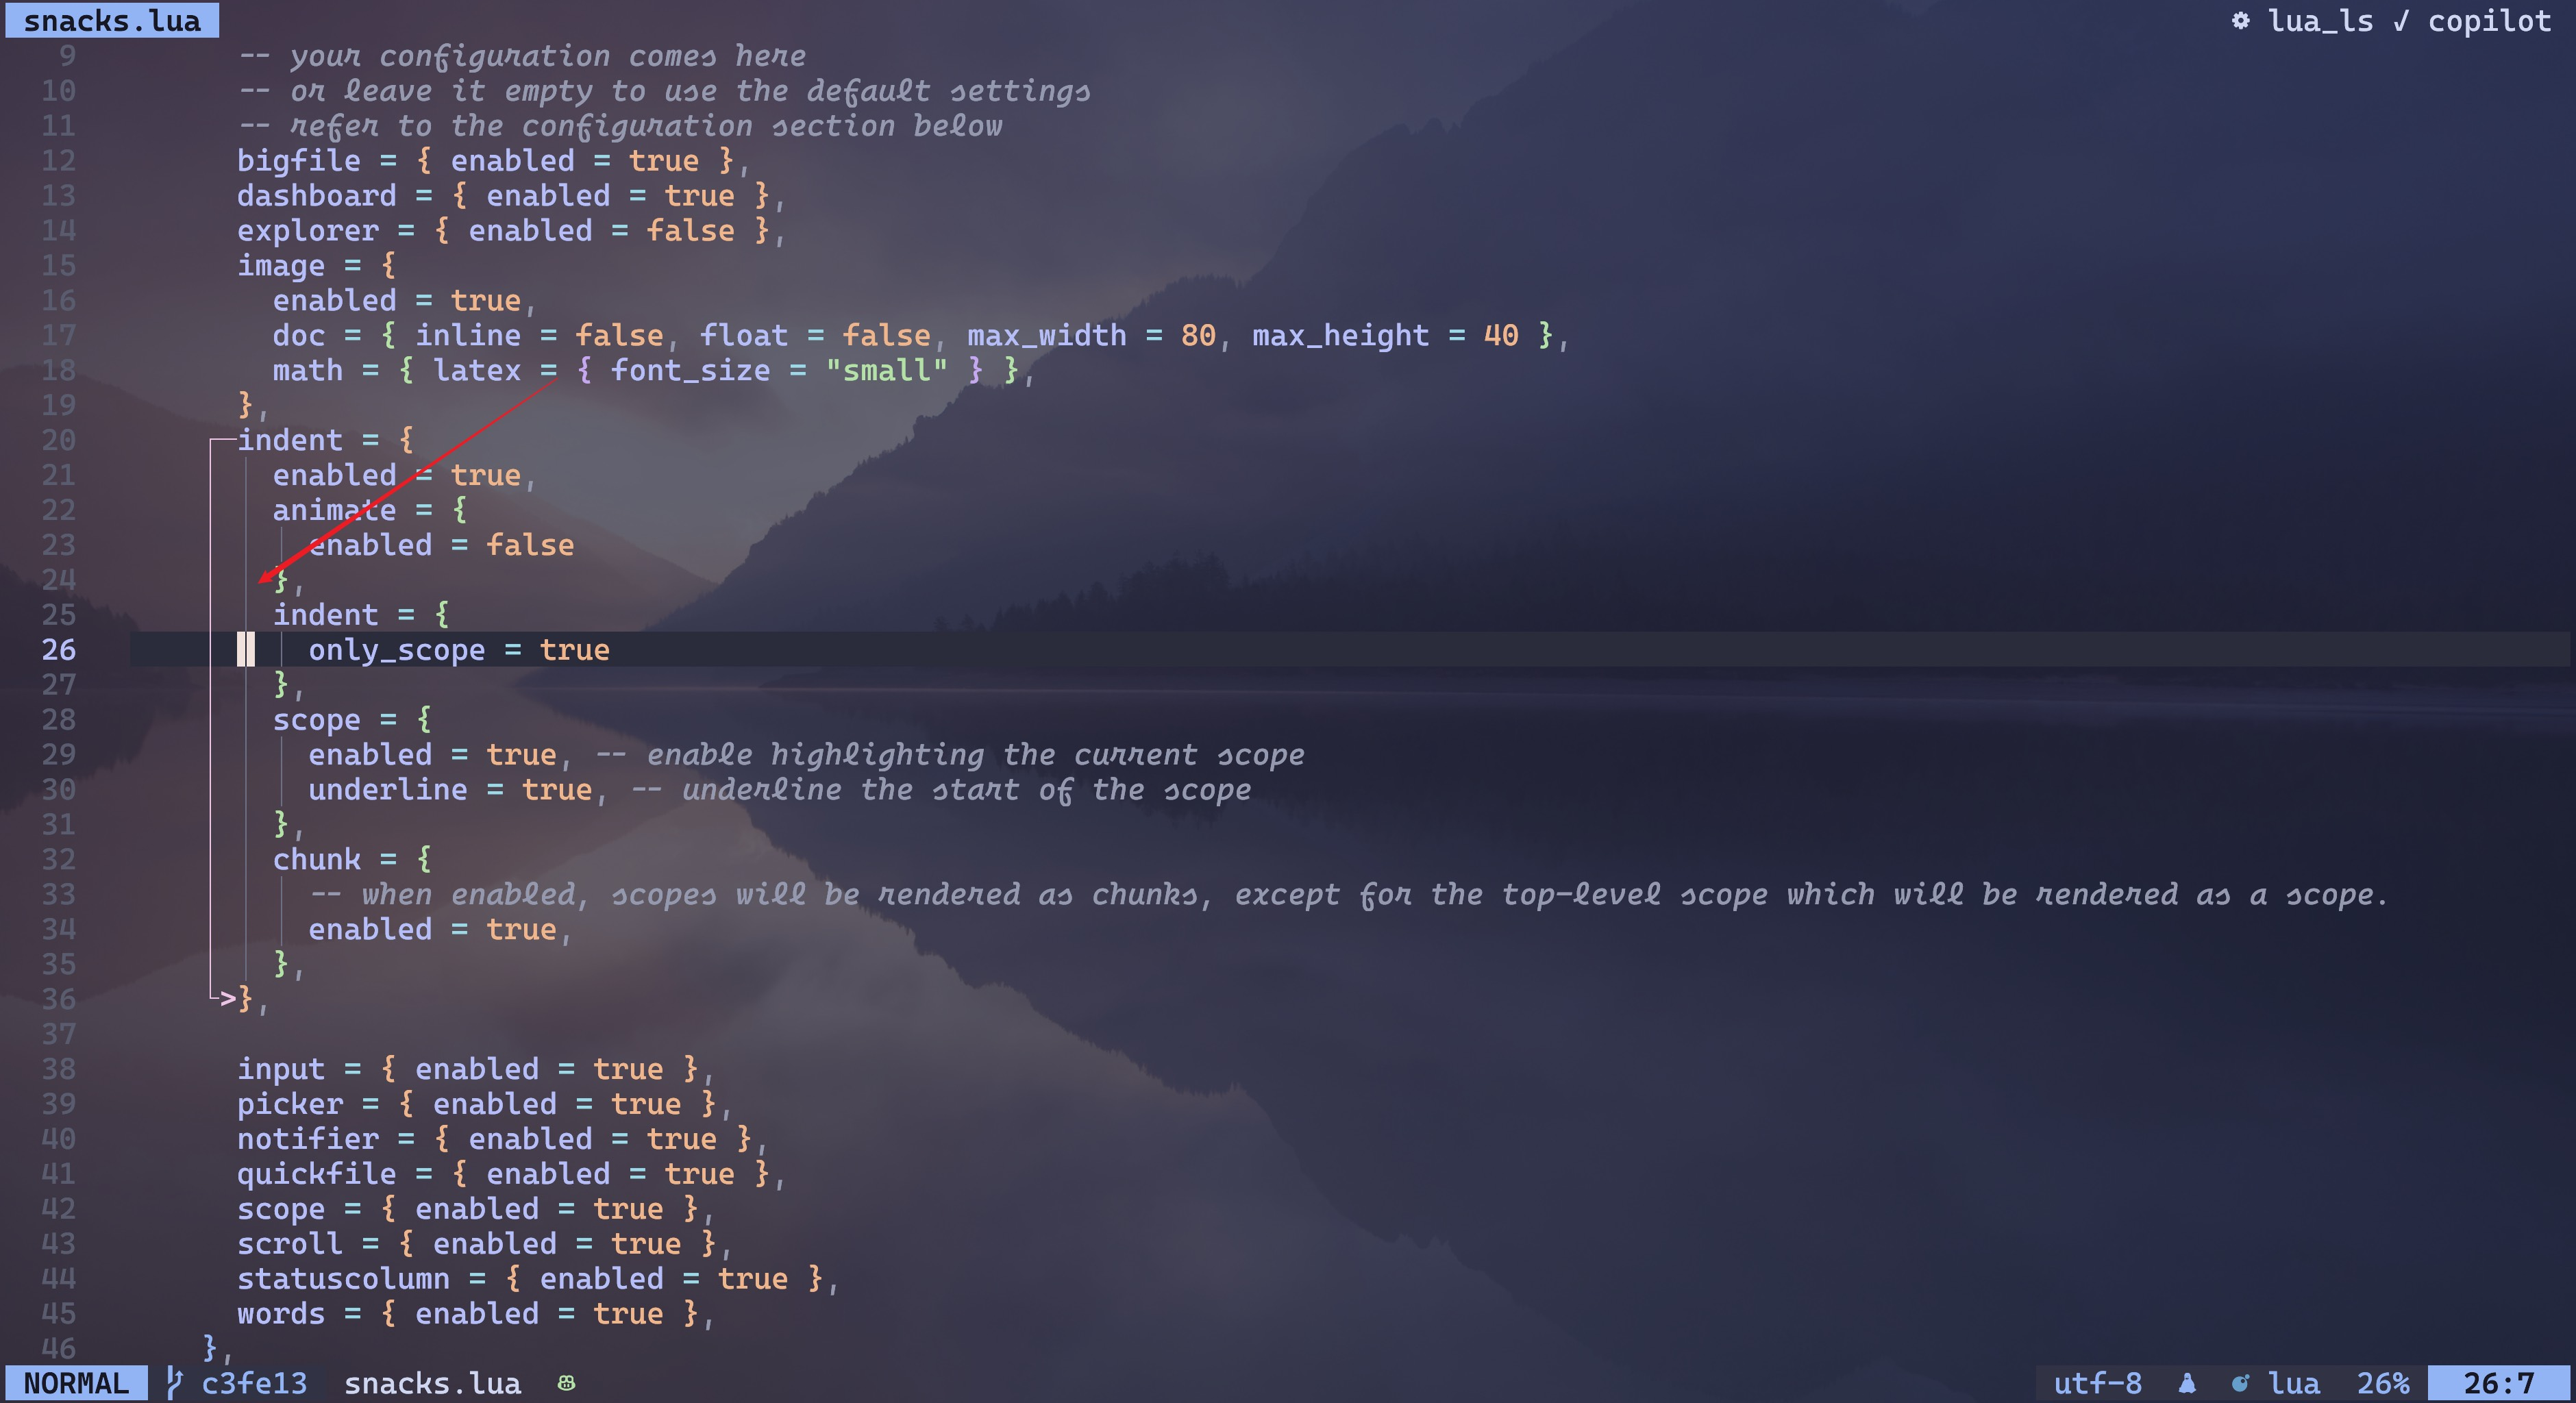
\includegraphics[width=0.7\linewidth]{./Figures/Snacks_Config_4_Indent.jpg}
        \end{figure}
    \end{itemize}
  \end{frame}

  \begin{frame}{snacks.nvim}
    \begin{itemize}
      \item Lazygit窗口
        \begin{figure}[H]
          \centering
          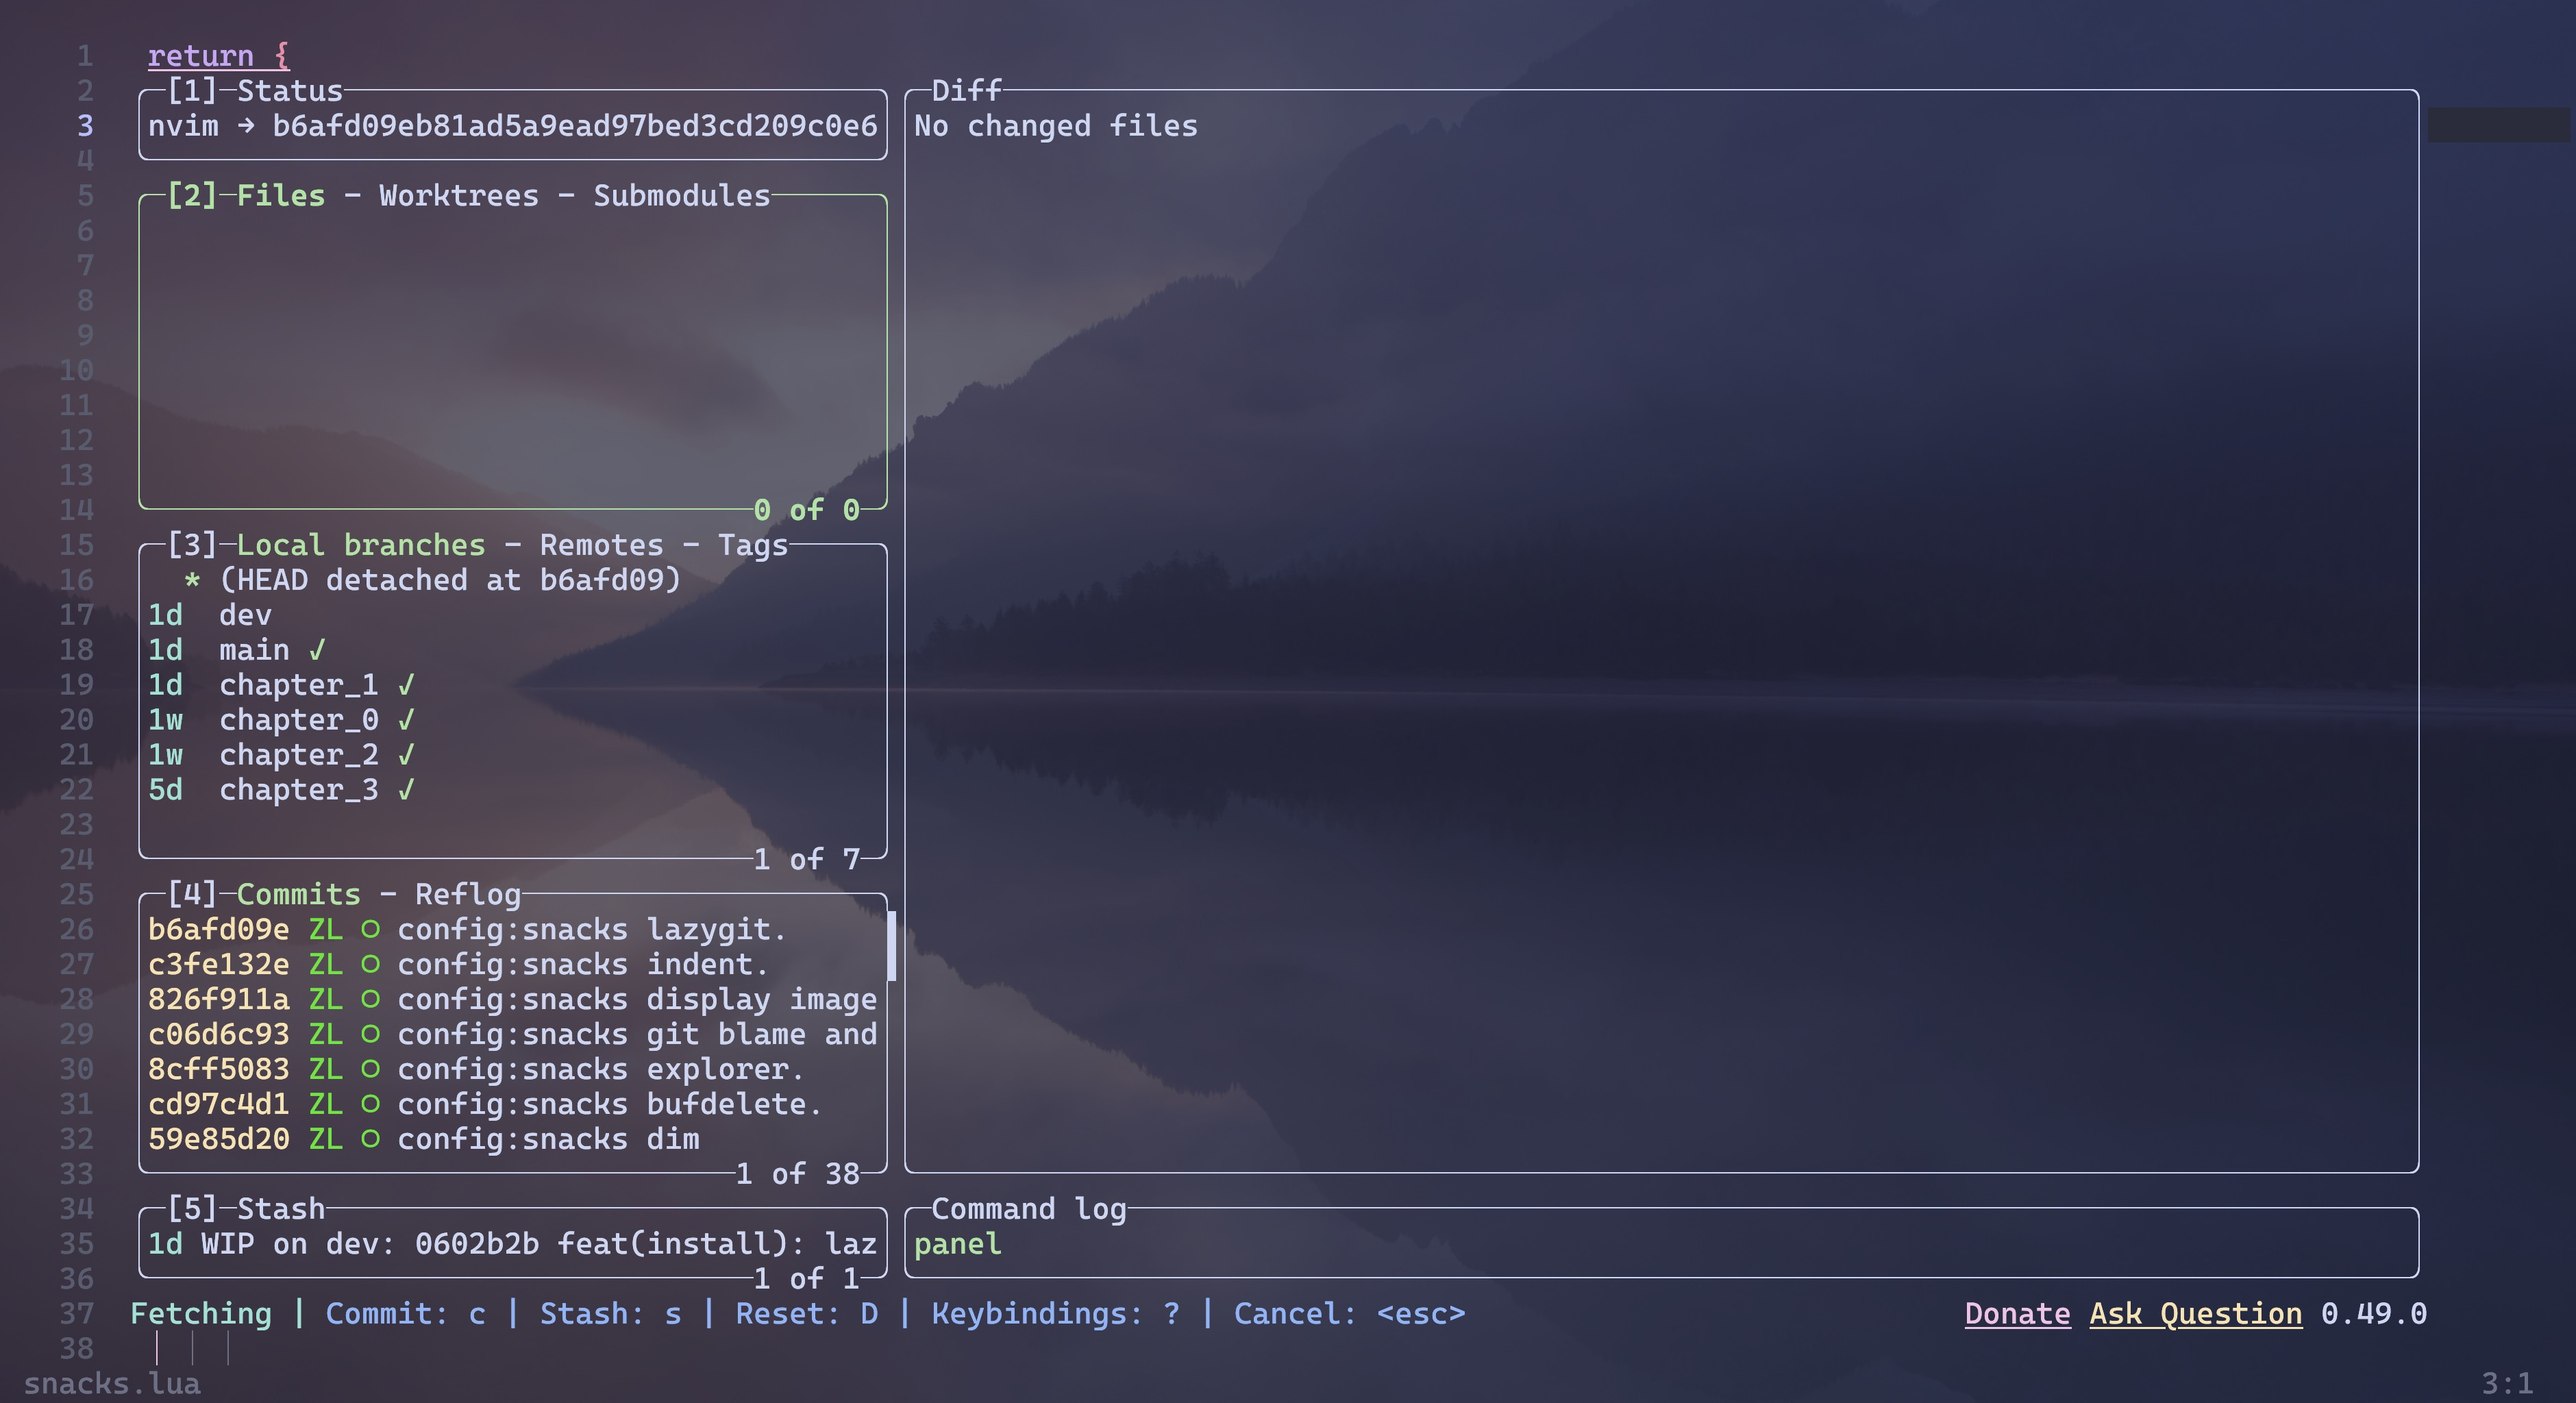
\includegraphics[width=0.7\linewidth]{./Figures/Snacks_Config_5_Lazygit.jpg}
        \end{figure}
    \end{itemize}
  \end{frame}

  \begin{frame}{snacks.nvim}
    \begin{itemize}
      \item Notifier
        \begin{itemize}
          \item 将原来使用的nvim-notify换成了snacks的notifier
        \end{itemize}
        \begin{figure}[H]
          \centering
          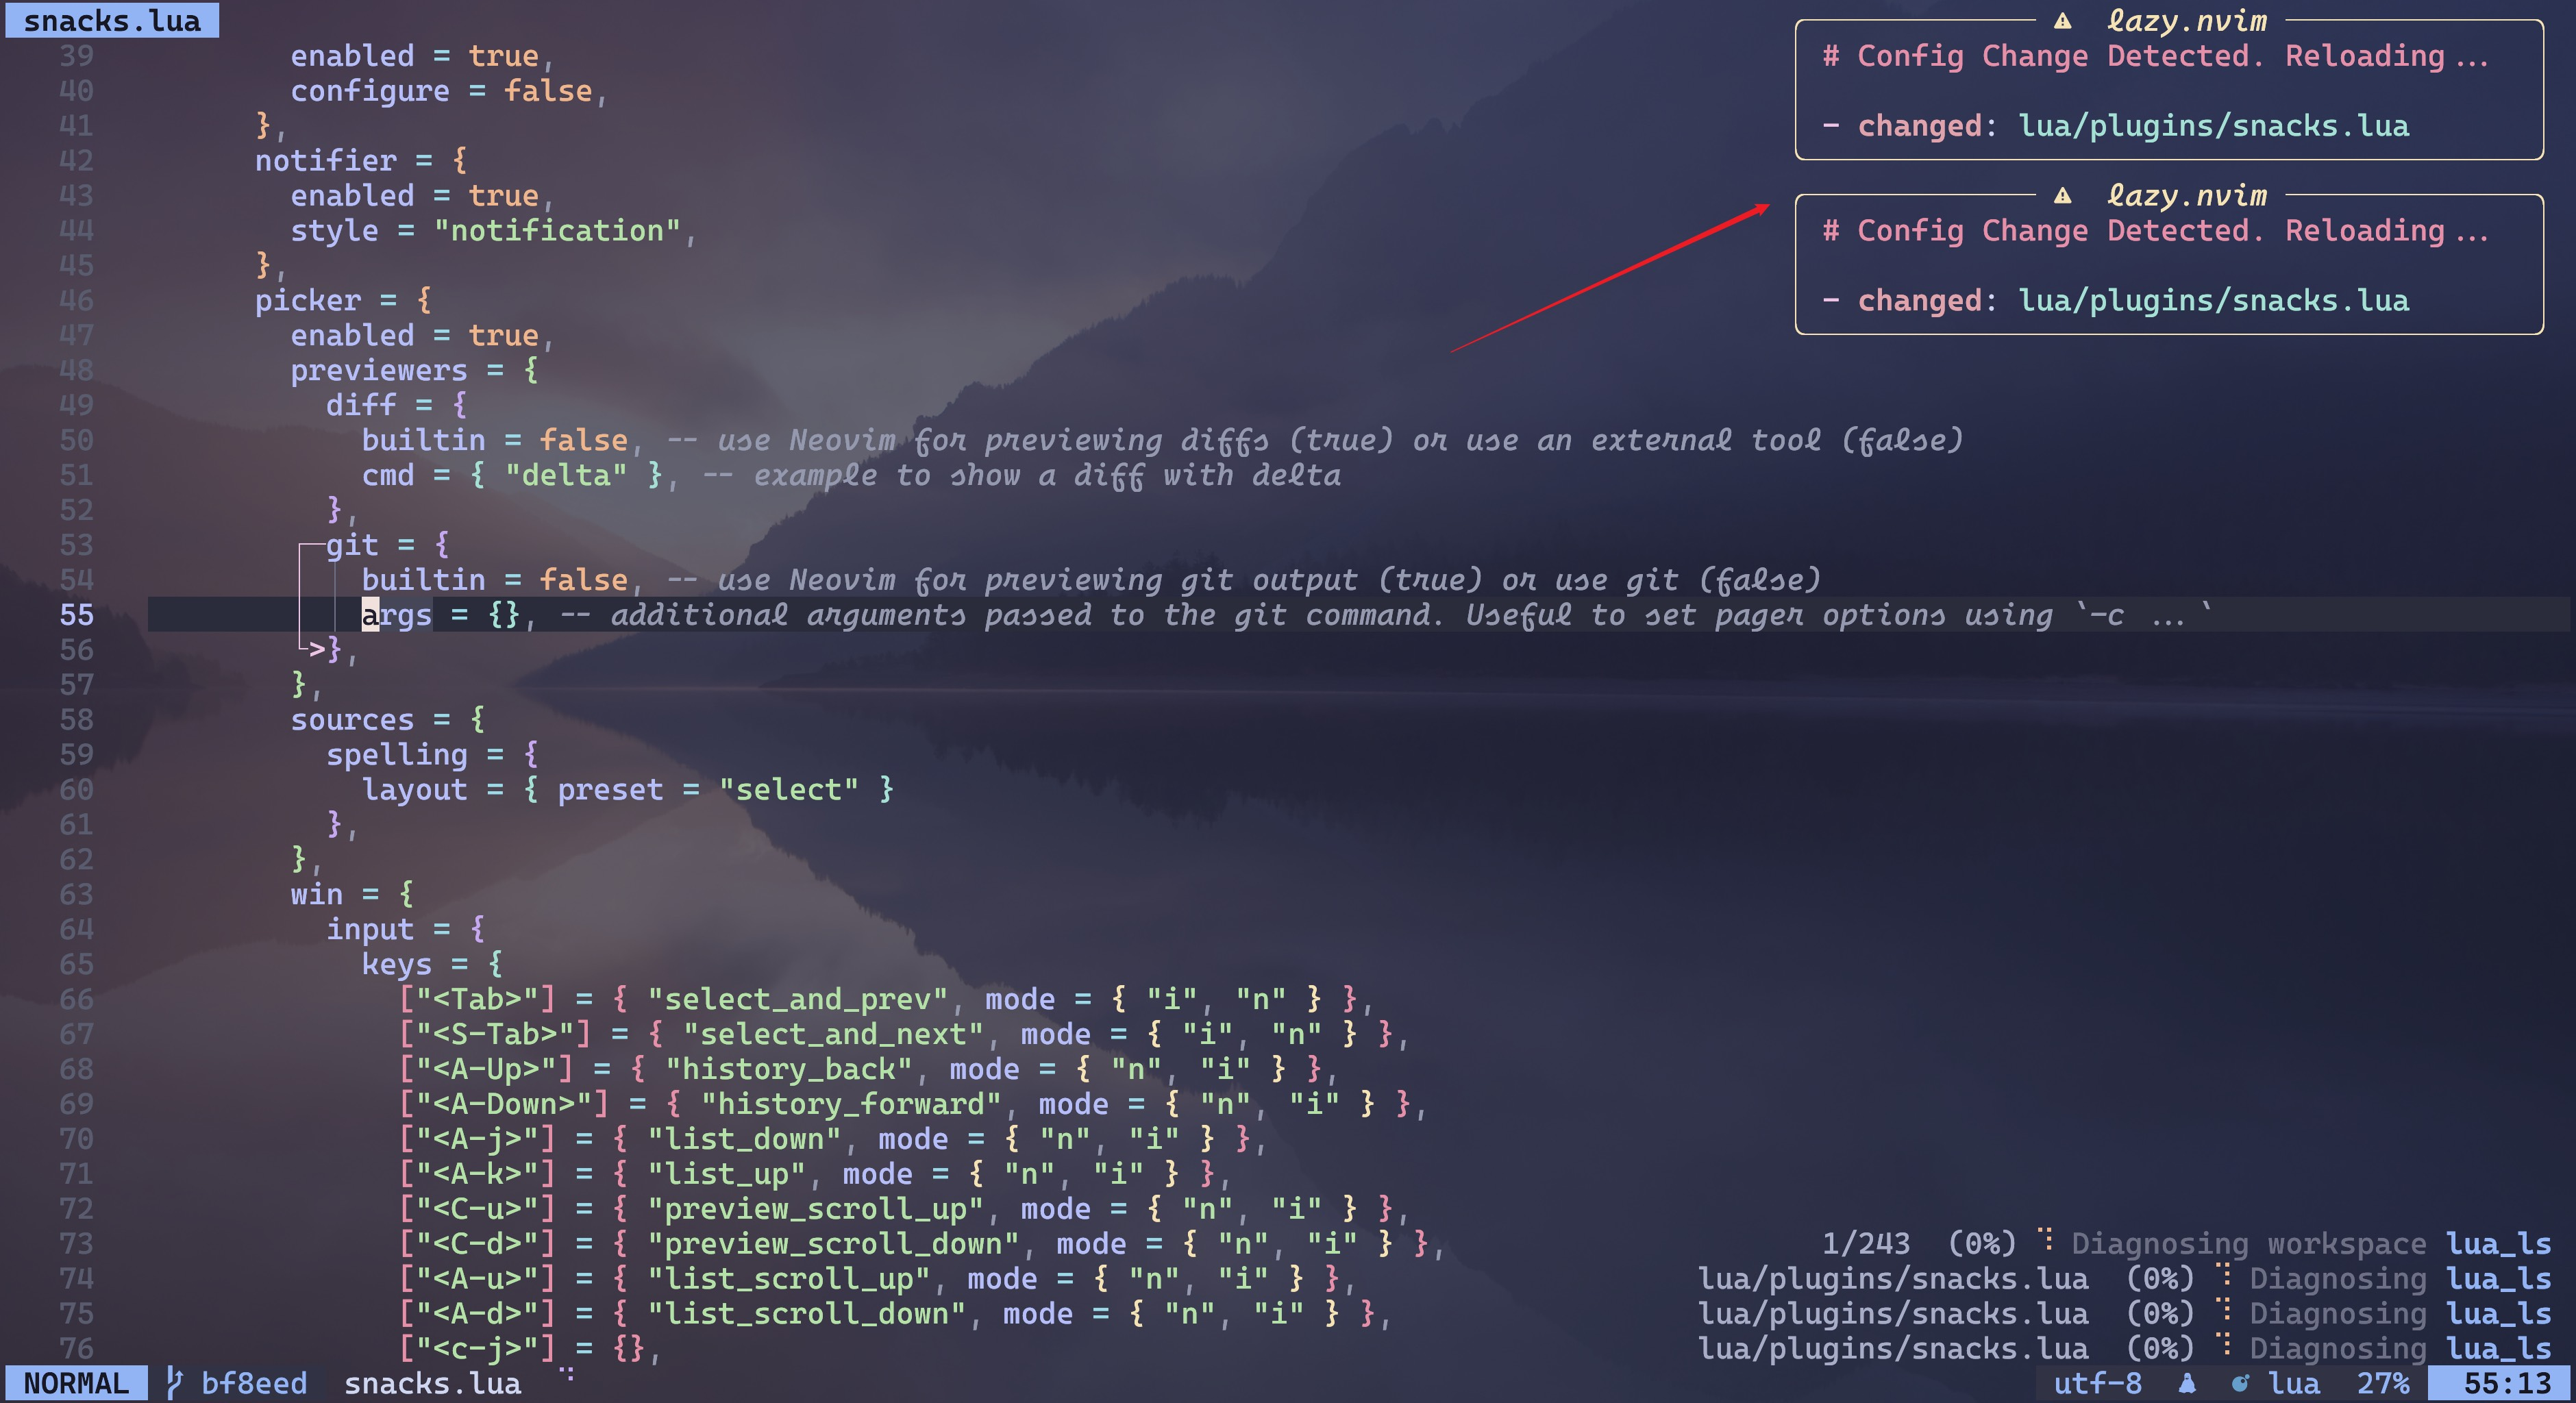
\includegraphics[width=0.7\linewidth]{./Figures/Snacks_Config_6_Notifier.jpg}
        \end{figure}
    \end{itemize}
  \end{frame}

  \begin{frame}{snacks.nvim}
    \begin{columns}
      \begin{column}{0.4\linewidth}
        \begin{itemize}
          \item 内容选择器(picker)
            \begin{itemize}
              \item 前置条件
                \begin{itemize}
                  \item ripgrep:文本搜索 % ChkTeX 19
                  \item git-delta:更好的git diff显示 % ChkTeX 19
                \end{itemize}
              \item 支持功能
                \begin{itemize}
                  \item 文件选择
                  \item 文本搜索 % ChkTeX 19
                  \item LSP相关选择
                  \item Git操作选择
                \end{itemize}
            \end{itemize}
        \end{itemize}
      \end{column}

      \begin{column}{0.6\linewidth}
        \begin{figure}[H]
          \centering
          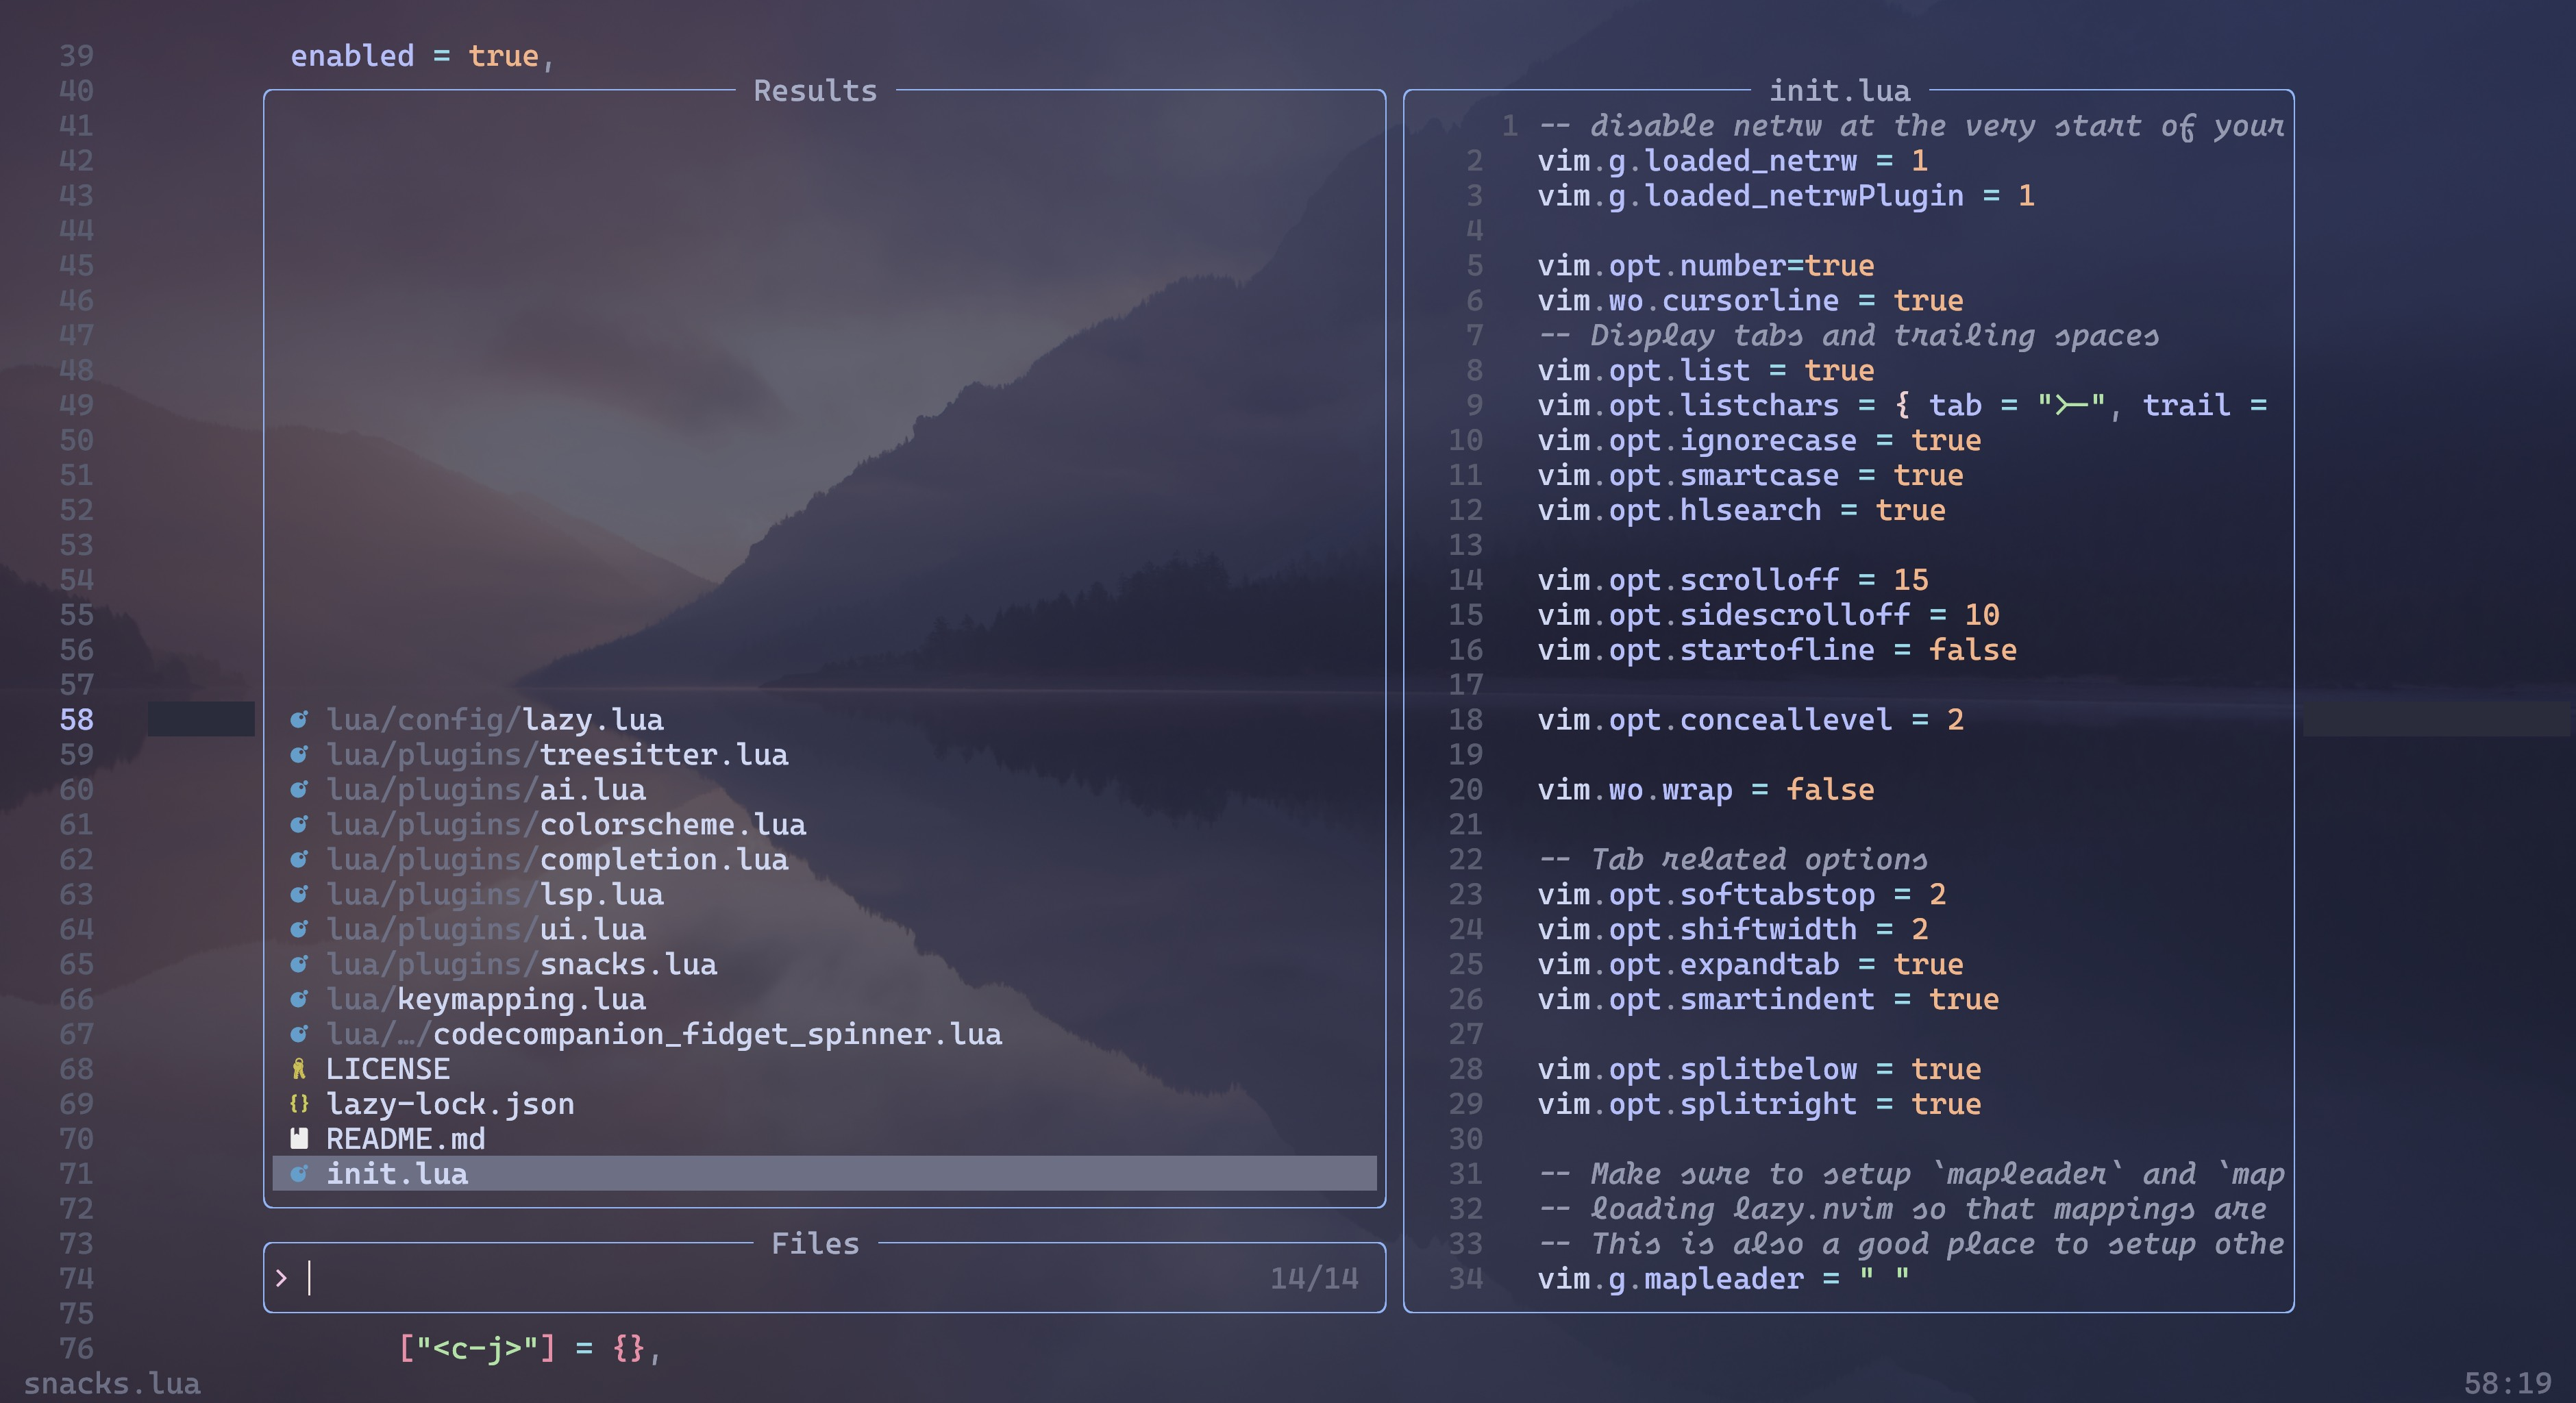
\includegraphics[width=\linewidth]{./Figures/Snacks_Config_7_Picker.jpg}
        \end{figure}
      \end{column}
    \end{columns}
  \end{frame}

  \begin{frame}{snacks.nvim}
    \begin{itemize}
      \item Profiler:neovim启动的性能分析
        \begin{figure}[H]
          \centering
          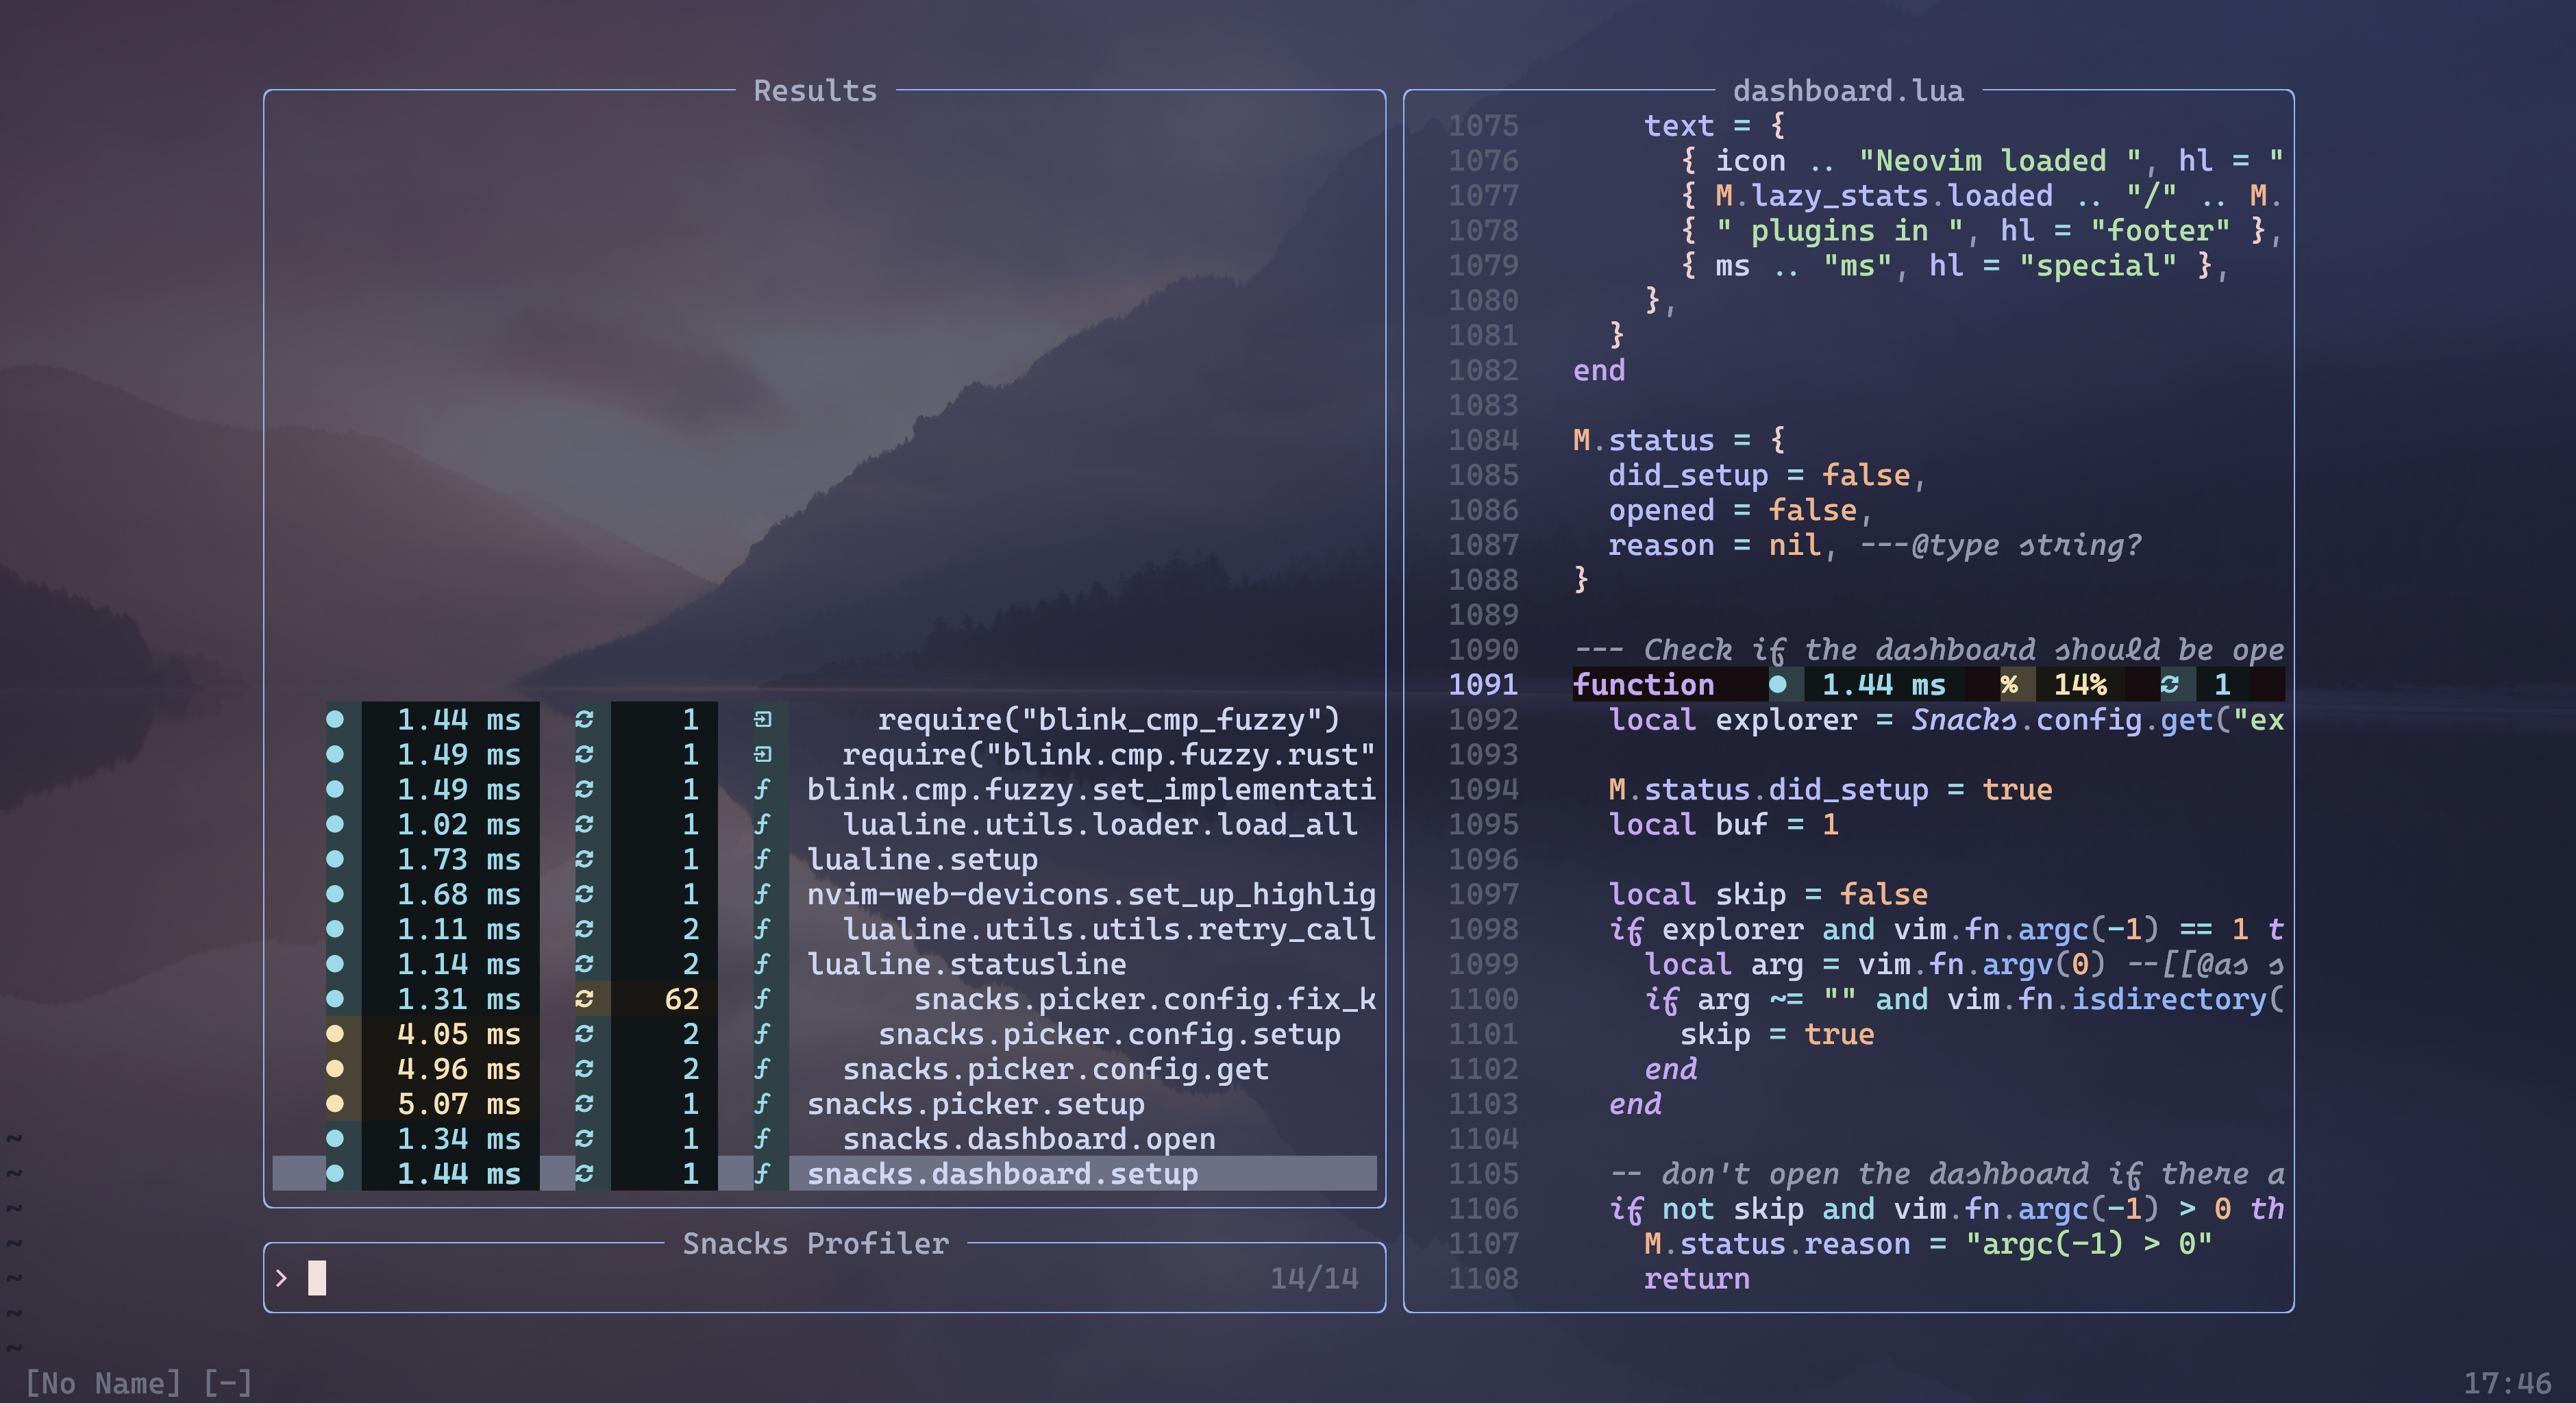
\includegraphics[width=0.7\linewidth]{./Figures/Snacks_Config_8_Profiler.jpg}
        \end{figure}
    \end{itemize}
  \end{frame}

  \begin{frame}{snacks.nvim}
    \begin{itemize}
      \item Scope:代码范围显示 % ChkTeX 19
        \begin{figure}[H]
          \centering
          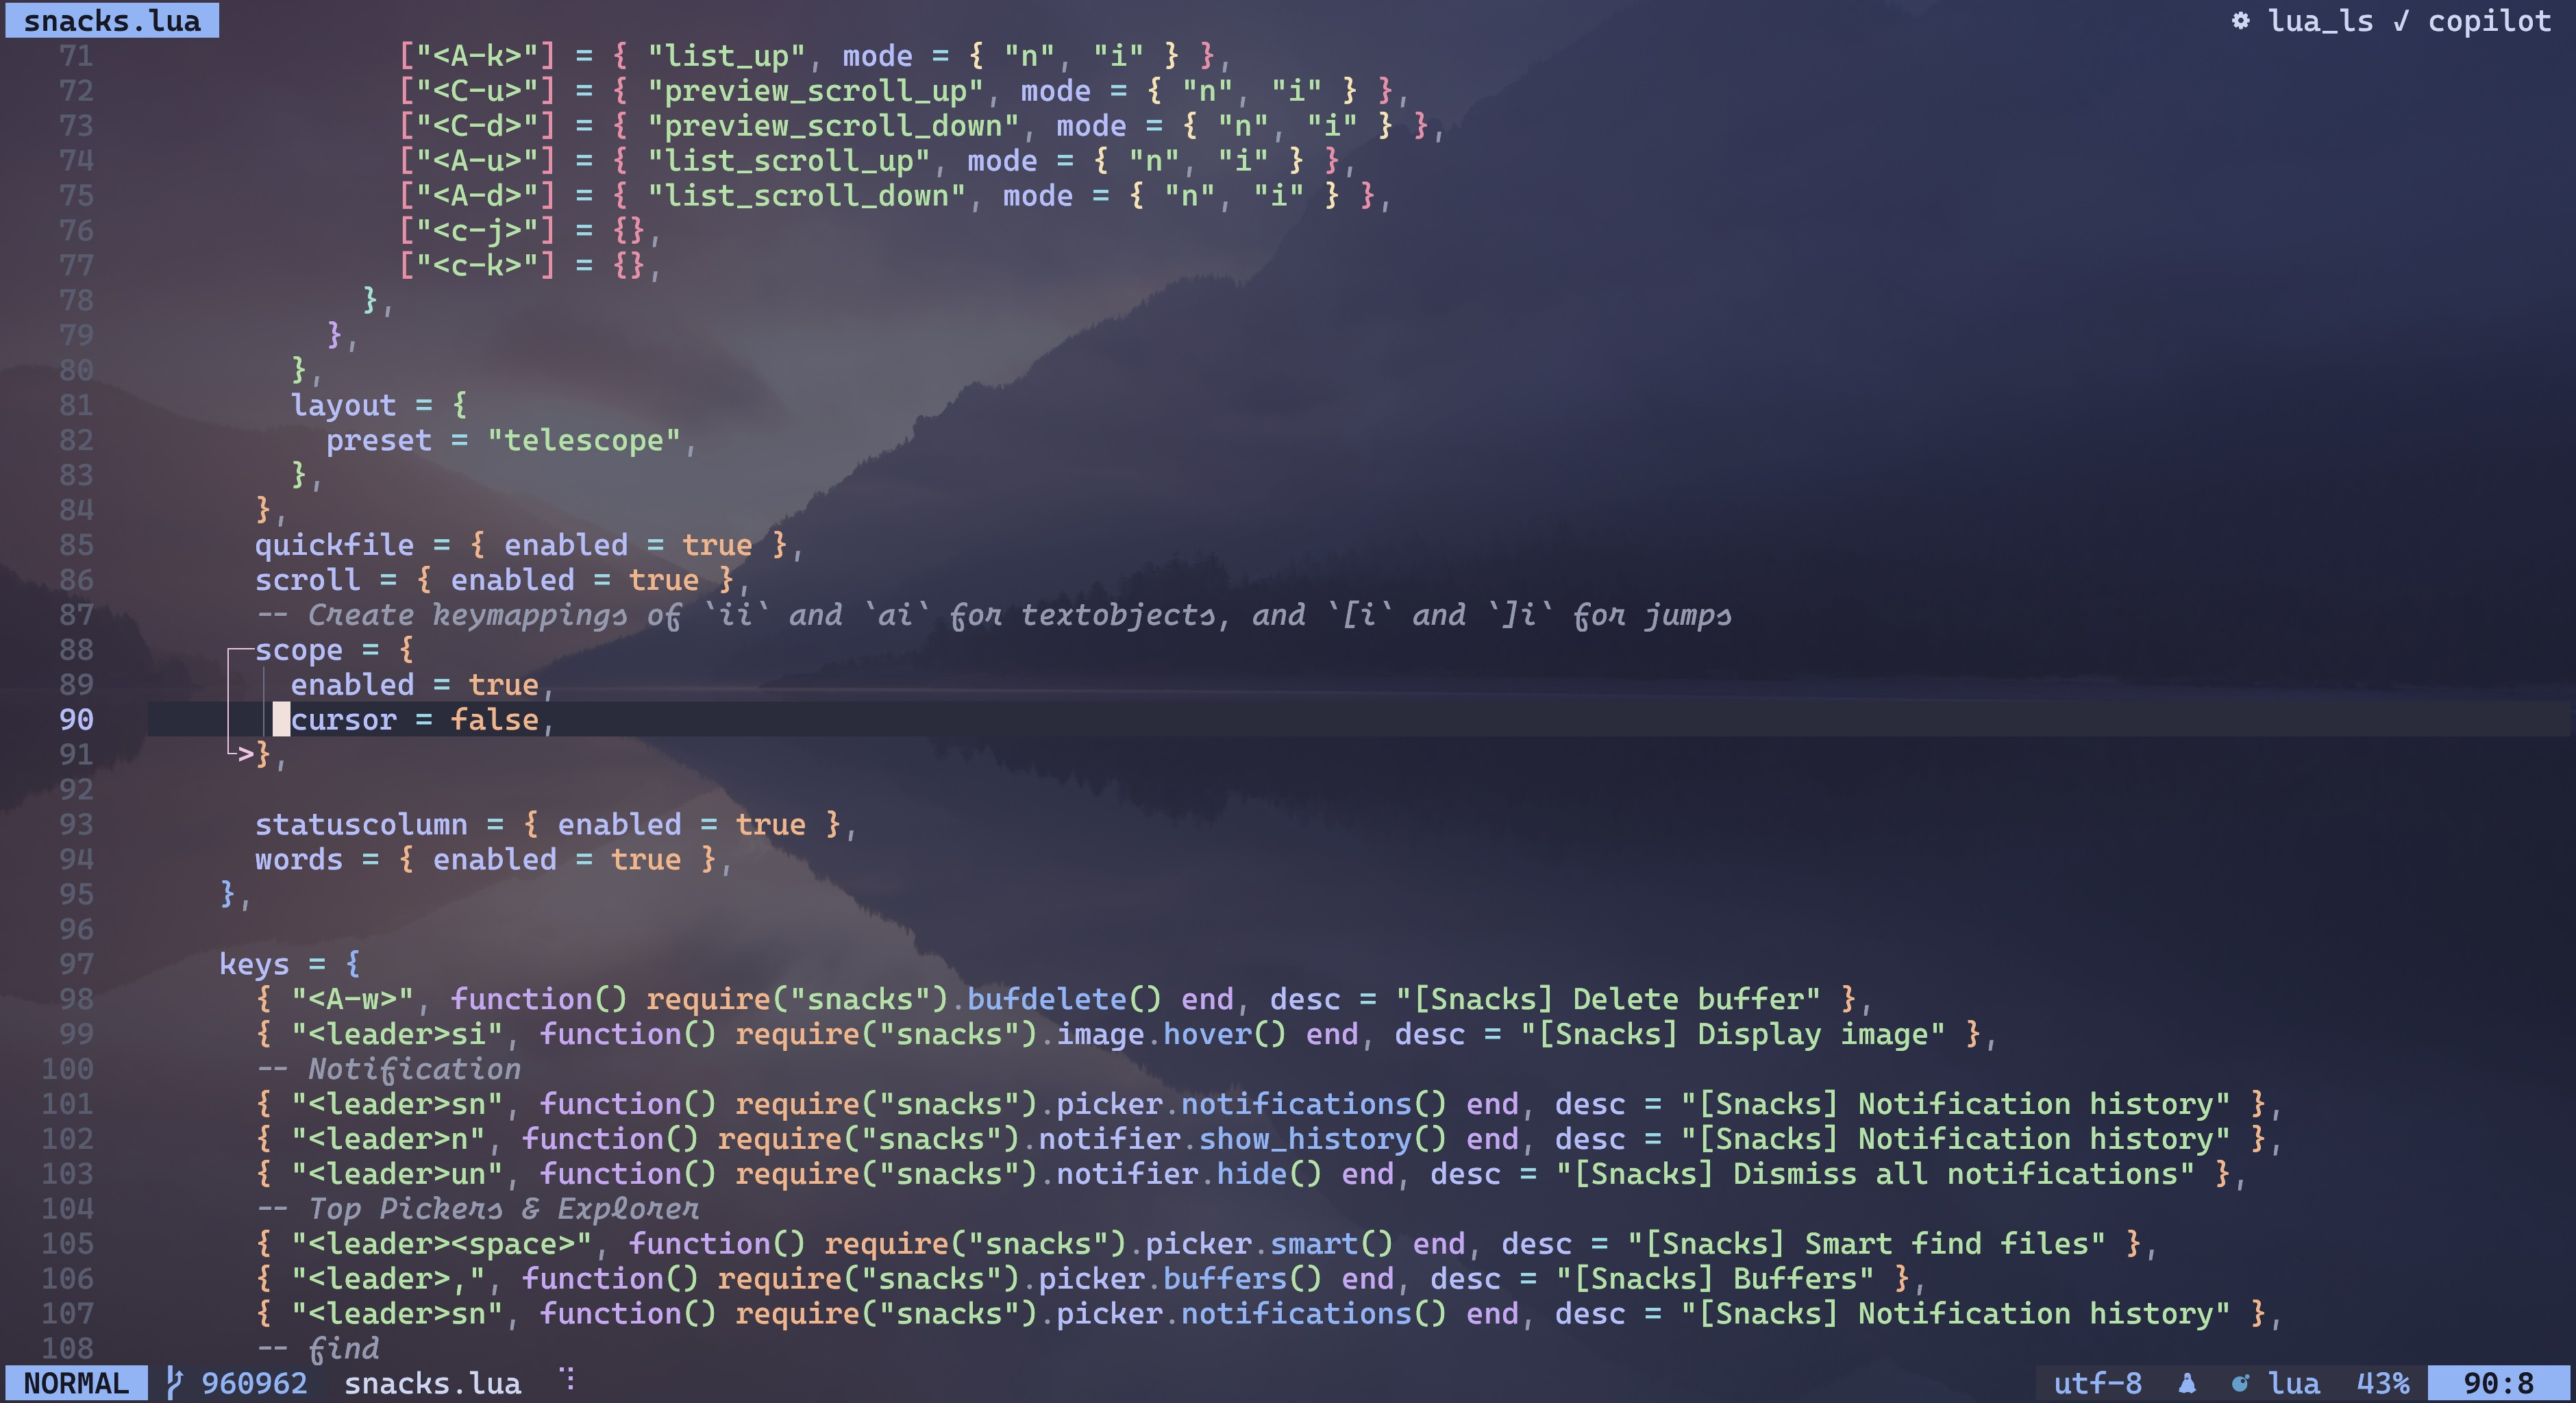
\includegraphics[width=0.7\linewidth]{./Figures/Snacks_Config_9_Scope.jpg}
        \end{figure}
    \end{itemize}
  \end{frame}

  \begin{frame}{snacks.nvim}
    \begin{itemize}
      \item 悬浮终端
        \begin{figure}[H]
          \centering
          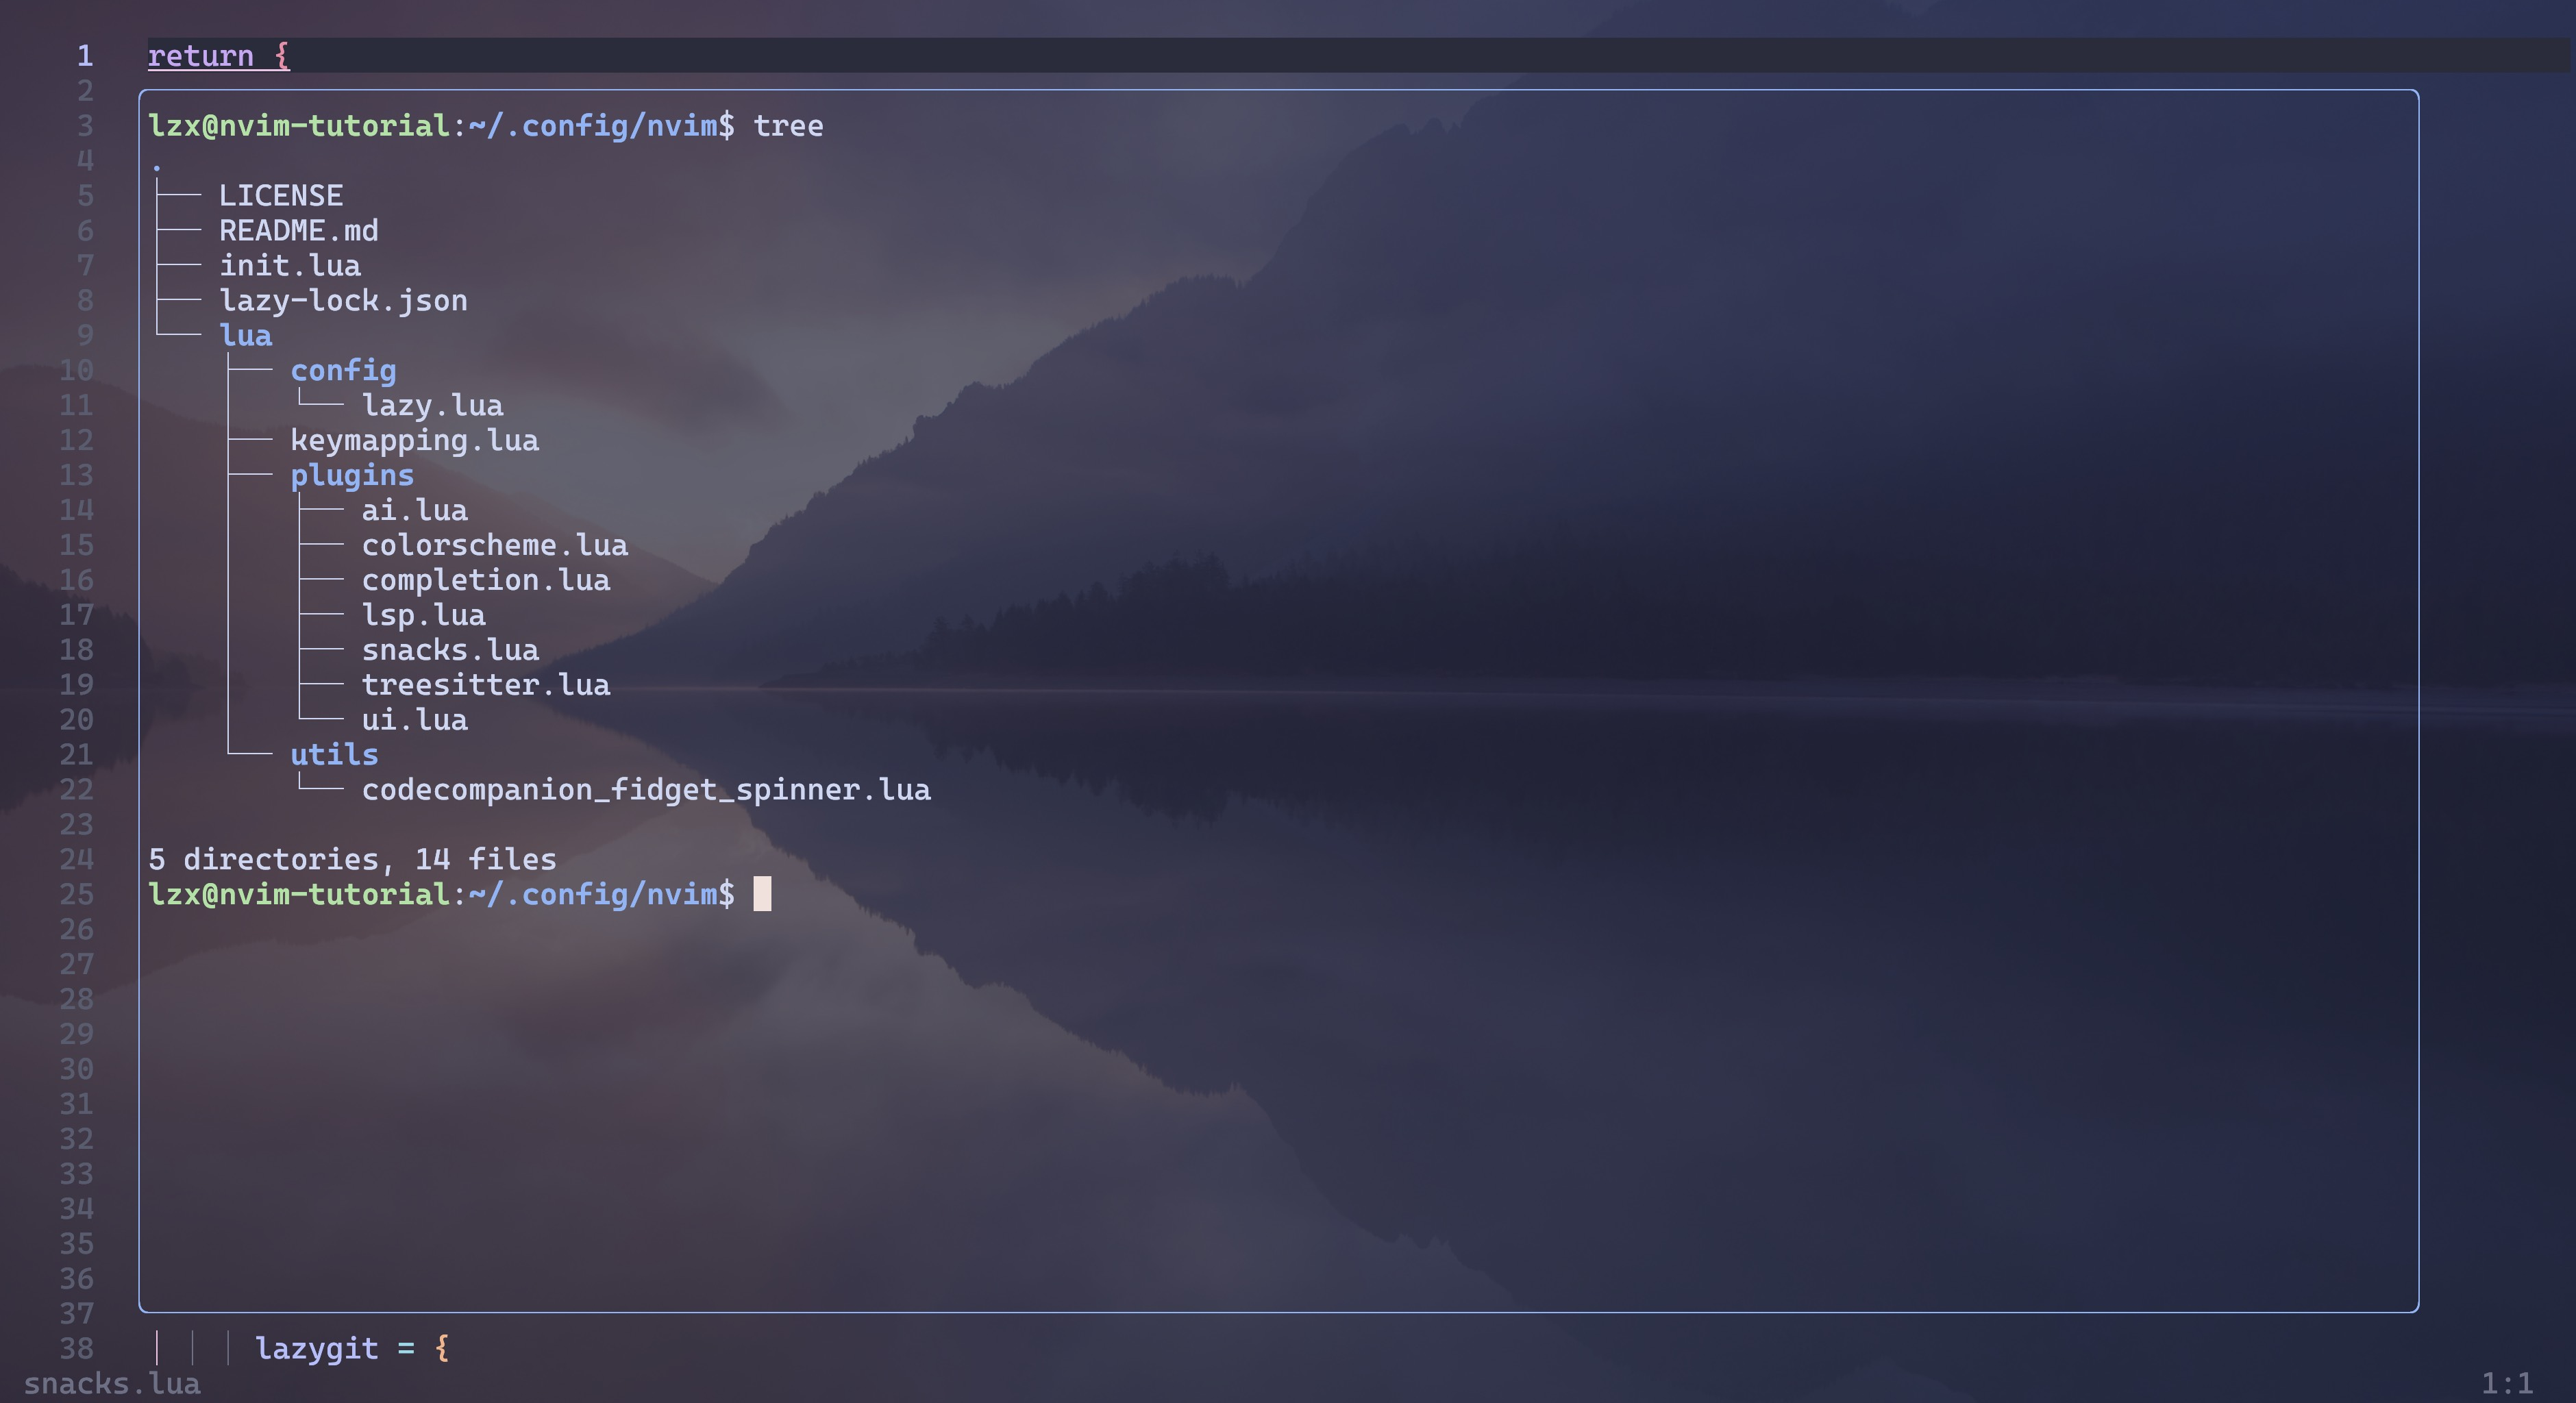
\includegraphics[width=0.7\linewidth]{./Figures/Snacks_Config_10_Terminal.jpg}
        \end{figure}
    \end{itemize}
  \end{frame}

  \begin{frame}{snacks.nvim}
    \begin{itemize}
      \item Zen mode:禅模式
        \begin{figure}[H]
          \centering
          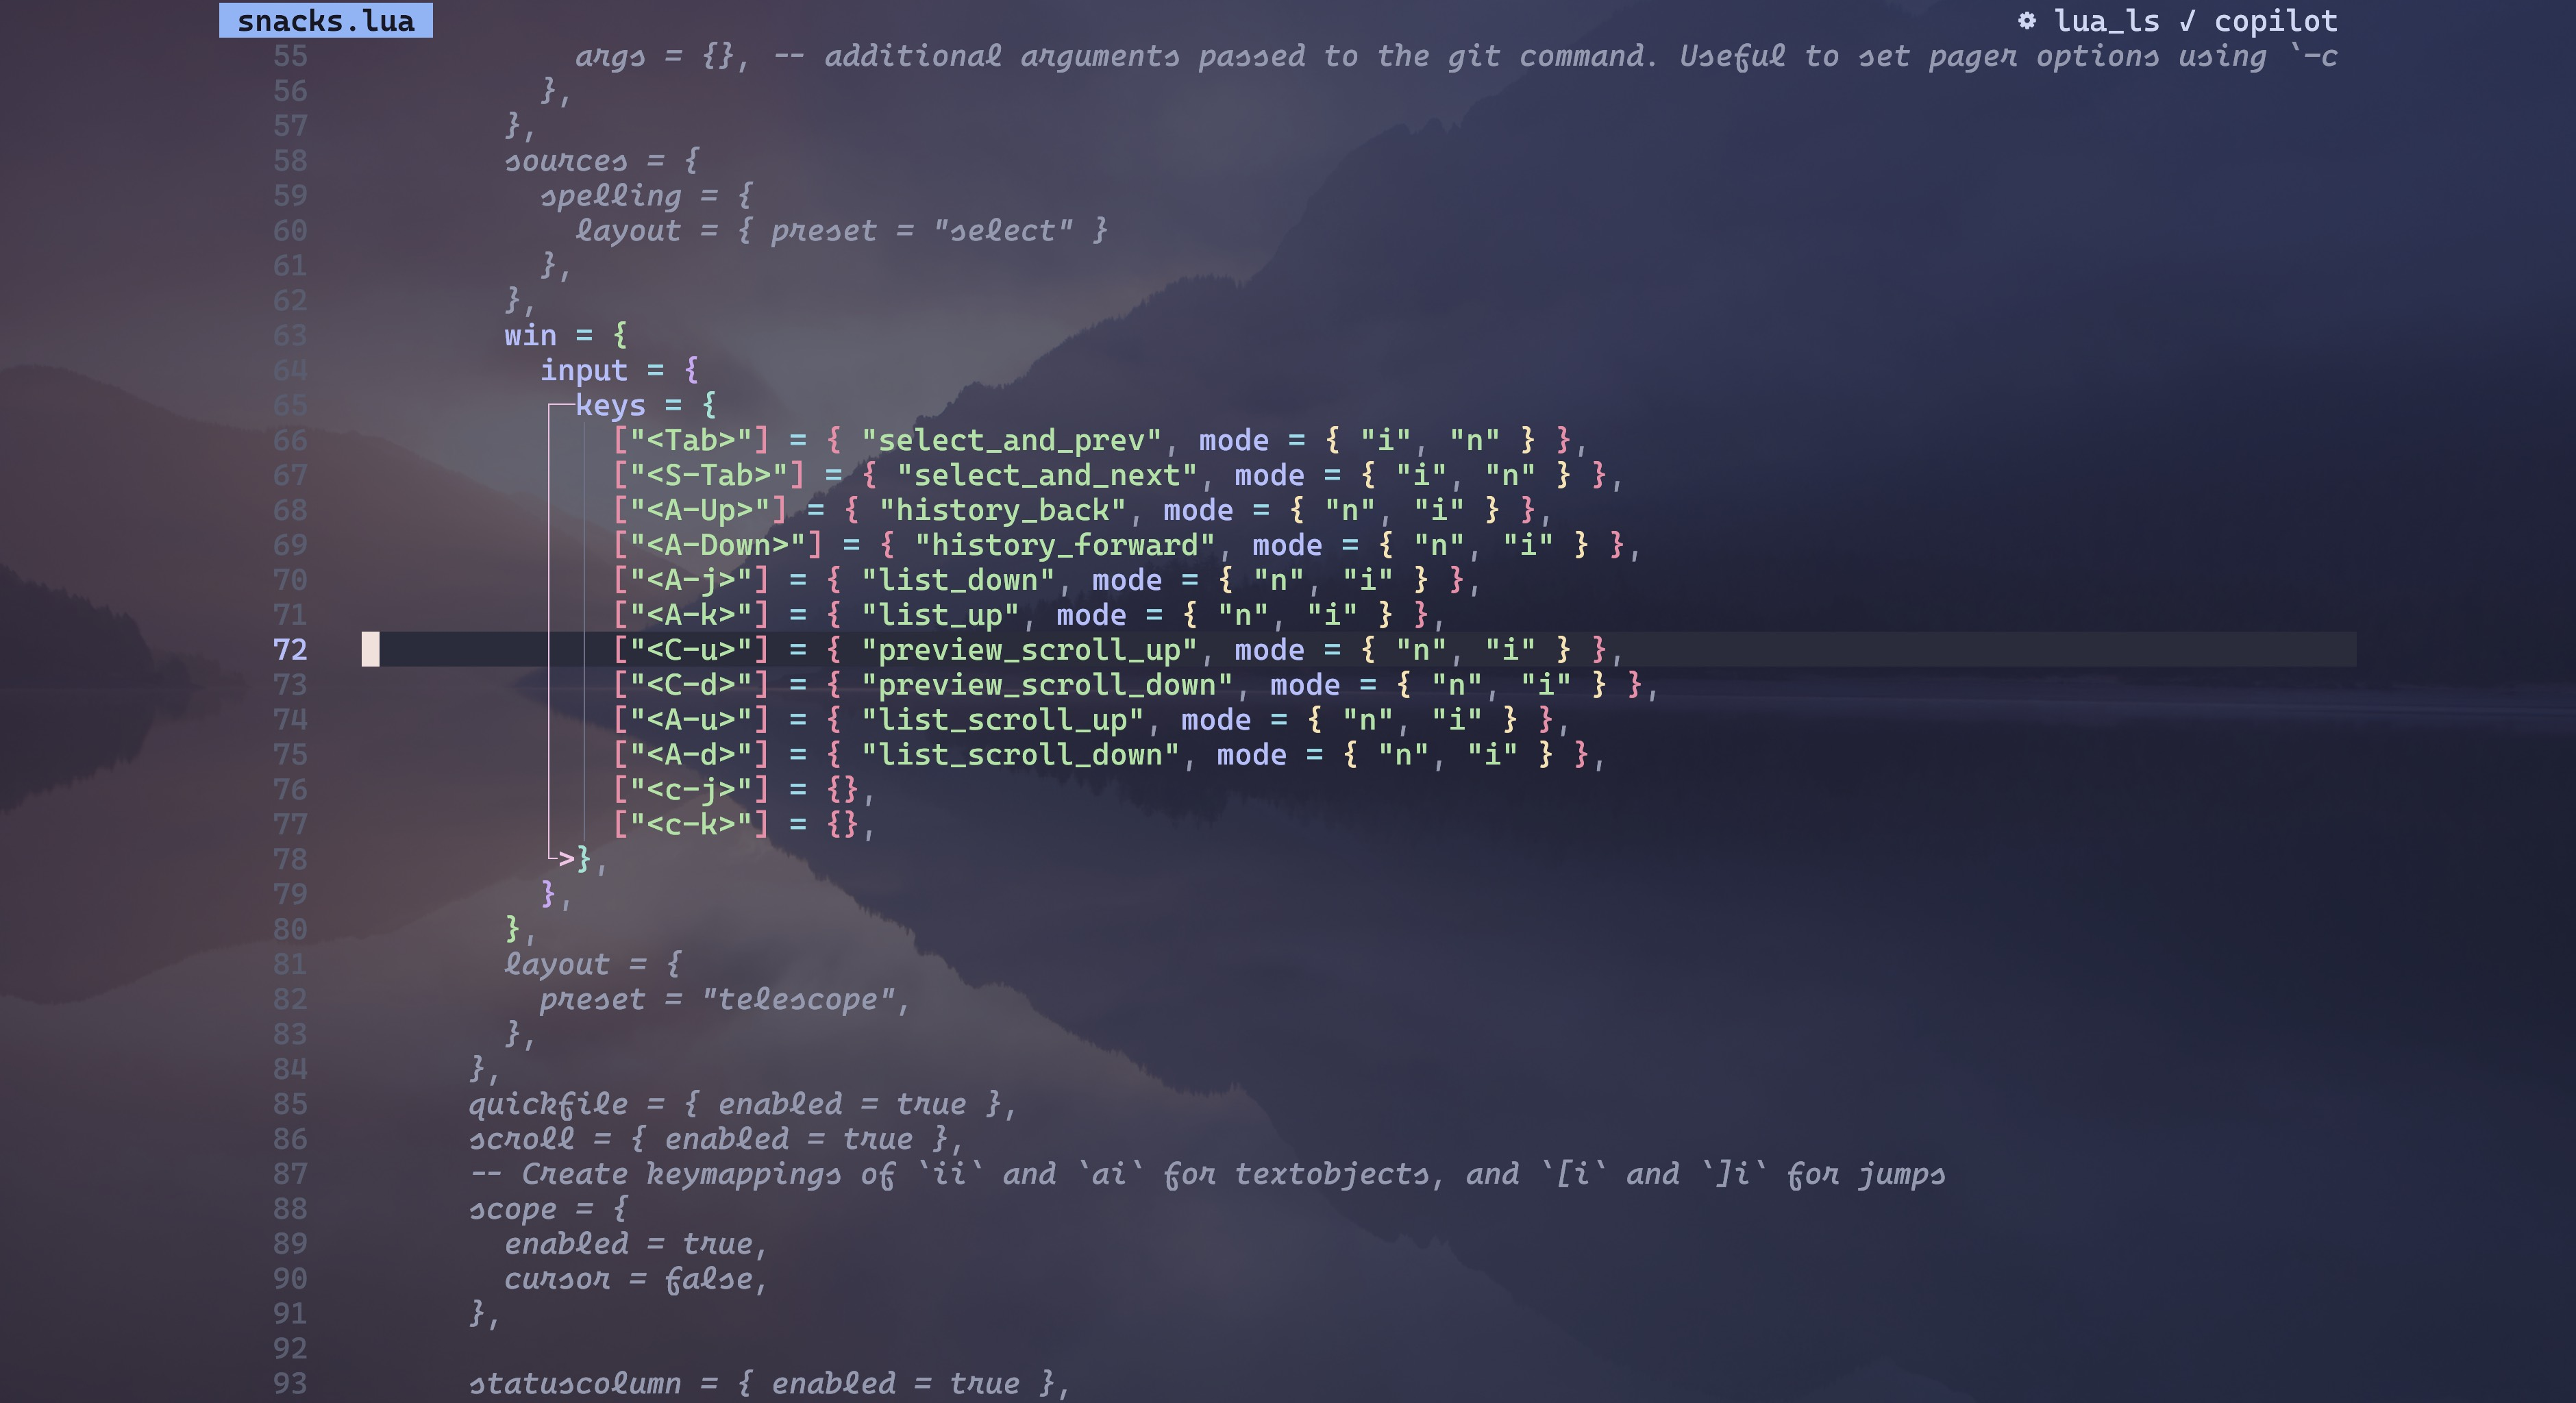
\includegraphics[width=0.7\linewidth]{./Figures/Snacks_Config_11_Zen.jpg}
        \end{figure}
    \end{itemize}
  \end{frame}

  \begin{frame}{snacks.nvim}
    \begin{itemize}
      \item 启用动画,禁用平滑滚动,添加切换快捷键
      \item \dots
      \item 其它一些小功能,请参考
        \begin{itemize}
          \item 官方文档:\url{https://github.com/folke/snacks.nvim?tab=readme-ov-file}
          \item 我的配置文件:\lstinline[language={}, style=path]{\~/.config/nvim/lua/plugins/snacks.lua}
        \end{itemize}
    \end{itemize}
  \end{frame}

  \begin{frame}
    \begin{itemize}
      \item 感谢:
        \begin{itemize}
          \item \link{Catppuccin}{https://catppuccin.com/} 
\includegraphics[height=10pt]{./Figures/Catppuccin_logo.png}
          \item \link{Catppuccin for beamer}{https://github.com/atticus-sullivan/beamercolortheme}
        \end{itemize}
        \vspace{0.5cm}
      \item 本教程的全部材料可以在我的Github上找到
        \begin{itemize}
          \item Slides: \url{https://github.com/Jacky-Lzx/nvim.tutorial.slides}
          \item Config: \url{https://github.com/Jacky-Lzx/nvim.tutorial.config}
        \end{itemize}
    \end{itemize}
  \end{frame}

\end{document}
